\cotefile{36}
\scanpage{3}
\mspage{1}
\margin{\figure{\begin{tikzpicture}\draw (0,0) .. controls (.1,-.2) and (.4,-.35) .. (.6,-.65);\end{tikzpicture}}}

\uline{Remarques.\qquad SGA 7 $\boxed{\mathrm{IX}}$}

0.

i).\quad Dire que $\ell$ est un nombre premier à $p$ (pour que $\ell\,6$ soit OK p.e.)

Pourquoi $S$ \unsure{hensélien|Limélien} ?
\margin{$\ell\,7$\quad ii) $\ell\,3$}

$0.1,\ \ell\,9$ : pourquoi seulement à isogénie près ? (si $\ell\ne p$ : sinon ce ne veut rien dire)

$\ell\,14$ : il semble clair\qquad est un peu optimiste.

ii).\quad $\ell\,14$\quad français :\qquad et qui\qquad ($\,;\,$ il\quad ?)

iii).\quad
\figure{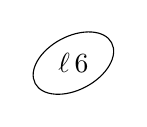
\begin{tikzpicture}[baseline=(t.base)]\node[inner sep=3pt] (t) {$\ell\,6$};\draw[rotate=28] (0,0) ellipse (0.55 and 0.34);\end{tikzpicture}}
une référence ou définition pour réduction semi-stable d'une courbe (seule la terminologie de ``réduction stable'' se trouve dans [3])

iv)\quad $\ell\,12$\quad orthographe ?\qquad \unsure{système}

\figure{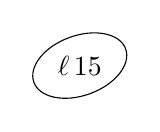
\begin{tikzpicture}[baseline=(t.base)]\node[inner sep=3pt] (t) {$\ell\,15$};\draw[rotate=20] (0,0) ellipse (0.62 and 0.38);\end{tikzpicture}}
vider la Rmq sur les $H^i$ (qui n'est ni
\figure{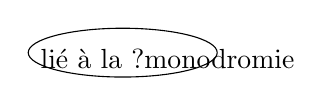
\begin{tikzpicture}[baseline=(t.base)]\node[anchor=west,inner sep=0pt] (t) at (0,0) {lié à la \inserted{?}monodromie};\draw (1.05,0.08) ellipse (1.20 and 0.31);\end{tikzpicture}}, ni fondé sur des théorèmes)

\figure{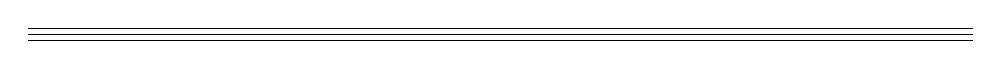
\begin{tikzpicture}\draw (0,0)--(12,0);\draw (0,-0.08)--(12,-0.08);\draw (0,-0.16)--(12,-0.16);\end{tikzpicture}}

1.

\uline{p 0.}\quad titre :\qquad $\ell'$ (minuscule)

$(1.0)\ \ell\,5$\qquad donc\qquad ?

\figure{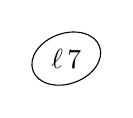
\begin{tikzpicture}[baseline=(t.base)]\node[inner sep=3pt] (t) {$\ell\,7$};\draw[rotate=20] (0,0) ellipse (0.45 and 0.32);\end{tikzpicture}}
à quel concept se rapporte ``lequel''.

\rule{\linewidth}{0.3pt}

\uline{p.1}\quad $\ell\,12$\quad français : choisie\quad ; ``qui est'' tend à faire croire qu'on impose une condition supplémentaire

$\ell\,16$\quad $=B$ donc le symbole est \unsure{malheureux};\quad $=A'_K$ de toute façon.

\rule{\linewidth}{0.3pt}

p2\quad $\ell\,2$\quad pourquoi
\figure{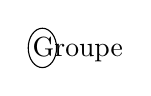
\begin{tikzpicture}[baseline=(t.base)]\node[anchor=west,inner sep=0pt] (t) at (0,0) {Groupe};\draw (0.13,0.02) ellipse (0.18 and 0.25);\end{tikzpicture}}
\quad -- épimorphisme n'est pas la définition d'isogénie --

$\ell\,15$\quad -- supprimer séparé type fini au bénéfice du seul quasi projectif.

-- que $A\mathbin{\underset{S}{\times}}\operatorname{Spec}(K)\xrightarrow{\sim}A_K$ est une trivialité

\margin{2}

\scanpage{4}
\mspage{2}
\margin{\figure{\begin{tikzpicture}\draw (0,0)--(.6,-.65);\end{tikzpicture}}}

$\ell-8$\quad pourquoi\quad \uline{donc}\qquad ?

\rule{\linewidth}{0.3pt}

p3\quad $\ell-8,-9$\qquad $B$ ?

\rule{\linewidth}{0.3pt}

p4.\quad 1.3.1.\quad As tu vérifié si l'accouplement d'\unsure{A. M.} coïncide avec le tien ?

$\ell\,4$.\quad \uline{formellement} non ramifié ?

$\ell\,7$.\quad \uline{séparablement} clos ?

$\ell\,14-20$.\quad Est-ce utile à dire, en l'absence de référence à ce que ce peut vouloir dire ?

$\ell-5$\quad Qu'il soit\qquad et\qquad \unsure{signifierait}\qquad plutôt ?

\rule{\linewidth}{0.3pt}

pg5\quad $\ell-2$\quad français :\quad les classes $\unsure{w|\omega}$\qquad \uline{en}\qquad relatifs.

\rule{\linewidth}{0.3pt}

pg6\quad $\ell\,4$\quad français.\quad dire\quad un Module inversible simple\qquad ?

\deleted{\illegible{5}}

\figure{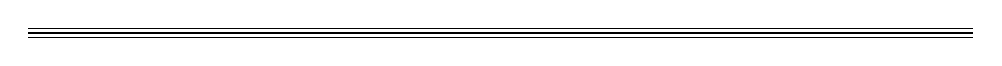
\begin{tikzpicture}\draw (0,0)--(12,0);\draw (0,-0.06)--(12,-0.06);\draw (0,-0.12)--(12,-0.12);\end{tikzpicture}}

\figure{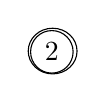
\begin{tikzpicture}[baseline=(t.base)]\node (t) {2};\draw (0,0) circle (0.27);\draw (0.01,0.01) ellipse (0.31 and 0.29);\end{tikzpicture}}

pg7\quad français \uline{$\ell-9$}\quad
\figure{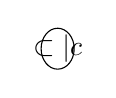
\begin{tikzpicture}[baseline=(t.base)]\node[inner sep=2pt] (t) {$\unsure{\subset|c}$};\draw (0,0) ellipse (0.21 and 0.26);\end{tikzpicture}}
$L_0$\quad donc
\figure{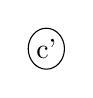
\begin{tikzpicture}[baseline=(t.base)]\node[inner sep=2pt] (t) {c'};\draw (0,0) ellipse (0.23 and 0.26);\end{tikzpicture}}
est

\deleted{$\ell\unsure{-8}$\quad \unsure{si}\quad \illegible{1}\quad \unsure{que}}
\quad $\ell-7$\quad
\figure{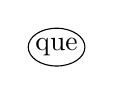
\begin{tikzpicture}[baseline=(t.base)]\node[inner sep=2pt] (t) {que};\draw (0,0) ellipse (0.36 and 0.24);\end{tikzpicture}}
(le $2^{\mathrm{e}}$)

\rule{\linewidth}{0.3pt}

pg8\quad français\quad $\ell\,4$\quad par exemple\quad à\inserted{\figure{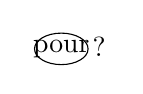
\begin{tikzpicture}[baseline=(t.base)]\node[inner sep=2pt] (t) {pour};\draw (0,0) ellipse (0.34 and 0.20);\node at (0.48,0.03) {?};\end{tikzpicture}}}\quad $\ldots$

$\ell-7$\quad \uline{le} terme

\rule{\linewidth}{0.3pt}

pg14.\quad L'argument est un peu immoral; si $X$ et $Y$ sont extensions d'une VA par un tore et si $\varphi:X\longrightarrow Y$ est donné, alors $\varphi$ est strictement compatible à la filtration par \unsure{le|les} poids et $\varphi$ est une isogénie si et seulement si $T_\ell(\varphi)$ en est une.

\rule{\linewidth}{0.3pt}

\figure{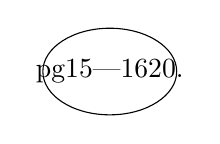
\begin{tikzpicture}[baseline=(t.base)]\node[inner sep=3pt] (t) {pg\deleted{\unsure{15|16}}20.};\draw (0,0) ellipse (0.85 and 0.55);\end{tikzpicture}}
Rmq 2.6 a)\quad $S$ est-il un trait dans cette remarque ; sait-on assez sur le passage à la limite et Néron ?

\margin{3}

\scanpage{5}
\mspage{3}
\margin{\figure{\begin{tikzpicture}\draw (0,0)--(.6,-.65);\end{tikzpicture}}}

\figure{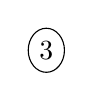
\begin{tikzpicture}[baseline=(t.base)]\node (t) {3};\draw (0,0) ellipse (0.23 and 0.28);\end{tikzpicture}}
\uline{pg23}\quad On peut dire plus simplement que ${}_nK$ est étale séparé car ${}_nK=\operatorname{Ker}({}_nG\longrightarrow{}_nH)$. En a), ne dirais-tu pas que ${}_nK_{\bar s}$ est isomorphe à un sous-groupe de ${}_nK_{\bar t}$.

\uline{pg24}\quad a) $\ell\,15$ :\quad
\figure{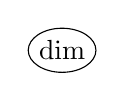
\begin{tikzpicture}[baseline=(t.base)]\node[inner sep=2pt] (t) {$\dim$};\draw (0,0) ellipse (0.43 and 0.28);\end{tikzpicture}}
$\operatorname{Ker}(u_{\unsure{\eta|s}})=0$\quad ?

\figure{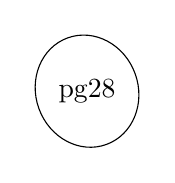
\begin{tikzpicture}[baseline=(t.base)]\node[inner sep=3pt] (t) {\uline{pg28}};\draw[rotate=20] (0,0) ellipse (0.65 and 0.72);\end{tikzpicture}}
Les notions introduites dans 3.5 ont elles été définies pour $S$ non hensélien ? (il faudrait au moins choisir un groupe d'inertie).
\inserted{[itou pour 3.7]}

\uline{pg29}\quad $\ell-2$\quad la terminologie ``clôture normale'' est-elle encore canonique ?

\figure{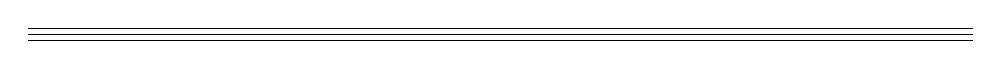
\begin{tikzpicture}\draw (0,0)--(12,0);\draw (0,-0.08)--(12,-0.08);\draw (0,-0.16)--(12,-0.16);\end{tikzpicture}}

\figure{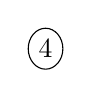
\begin{tikzpicture}[baseline=(t.base)]\node (t) {4};\draw (0,0) ellipse (0.22 and 0.26);\end{tikzpicture}}
\uline{p32}\quad $\ell\,8$\quad ne dépend
\figure{
\begin{tikzpicture}[baseline=(t.base)]\node[inner sep=2pt] (t) {pas};\draw (0,0) ellipse (0.28 and 0.27);\end{tikzpicture}}

\figure{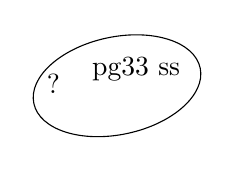
\begin{tikzpicture}[baseline=(t.base)]\node[inner sep=3pt] (t) {\uline{pg33 ss}};\node at (-1.05,-0.18) {?};\draw[rotate=12] (-0.28,-0.15) ellipse (1.08 and 0.62);\end{tikzpicture}}
(4.2)\quad Ne donnerais tu pas un énoncé style ``voisinage tubulaire'' compréhensible. La vérité est

\deleted{\unsure{a)}} on a un morphisme de topos $\operatorname{Spec}(K)_{\mathrm{et}}\xrightarrow{\varphi}\operatorname{Spec}(k)_{\mathrm{et}}$ (``\unsure{ext.|ent.} du corps résiduel'') et $A_0^0$ est un schéma relatif sur $(\operatorname{Spec}(\unsure{k|K}))_{\mathrm{et}}$ annelé par $\varphi^*\mathcal O$ [le $\varphi^*$ des faisceaux d'ensembles]. Même chose d'ailleurs pour
\figure{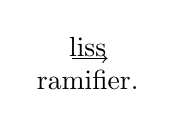
\begin{tikzpicture}[baseline=(t.base)]\node (t) at (0,0) {\unsure{liss}};\draw[->] (-0.2,-0.15)--(0.25,-0.15);\node at (0,-0.42) {\unsure{ramifier}.};\end{tikzpicture}}
$A_0$

\figure{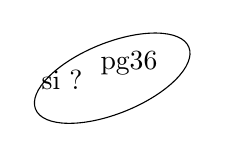
\begin{tikzpicture}[baseline=(t.base)]\node[inner sep=3pt] (t) {\uline{pg36}};\node at (-0.85,-0.22) {\unsure{si} ?};\draw[rotate=22] (-0.27,-0.10) ellipse (1.05 and 0.45);\end{tikzpicture}}
$\ell-6$.\quad ``ce n'est pas la trace qui est \unsure{contragrédiente}; l'énoncé primitif était correct.

\uline{pg40}\quad (4.5.4)\quad Qu'est-il écrit dans la marge ?

$\ell-1$\quad Quel est loc cit. ?

$\ell\,3$\quad $\ell$-groupe signifie-t-il tué par $\ell$, ou par un $\ell^{\unsure{n}}$ ?

Le trait est-il strictement local ? ce serait plus agréable.

\margin{4}

\scanpage{6}
\mspage{4}
\margin{\figure{\begin{tikzpicture}\draw (0,0) .. controls (.2,-.3) and (.5,-.45) .. (.6,-.7);\end{tikzpicture}}}

\figure{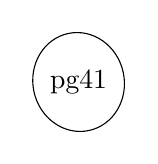
\begin{tikzpicture}[baseline=(t.base)]\node[inner sep=3pt] (t) {\uline{pg41}};\draw[rotate=12] (0,0) ellipse (0.58 and 0.63);\end{tikzpicture}}
$\ell-2$\quad ``fonction de Dirac'' est malheureux (sur un groupe, on ne \unsure{voit|sait} trop si c'est\quad ou
\diagram{\left\{\begin{array}{l} f(e)=1,\ 0\ \text{ailleurs}\\ f(e)=\#G,\ 0\ \text{ailleurs}\end{array}\right.})
\margin{\unsure{guillemets suffisent} ?}

\uline{pg42}\quad début dém. 4.7 : le \unsure{eps|cas} n'est pas clair pour $n=2$, et je n'ai pas confiance en dehors du cas strictement local.

\figure{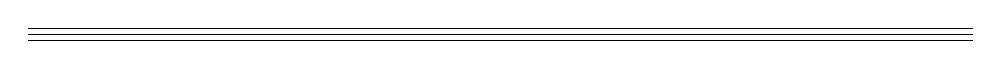
\begin{tikzpicture}\draw (0,0)--(12,0);\draw (0,-0.08)--(12,-0.08);\draw (0,-0.16)--(12,-0.16);\end{tikzpicture}}

\figure{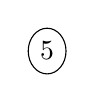
\begin{tikzpicture}[baseline=(t.base)]\node (t) {5};\draw (0,0) ellipse (0.24 and 0.29);\end{tikzpicture}}

\uline{pg\unsure{45|47}}\quad $\ell\,3$ ss\quad français : beaucoup de ``donc''.

\uline{pg46}\quad Quel est le sens de (5.2.3.1) et de \deleted{\unsure{le}} ``par définition'' qui suit --

S'agit-il de pro-objets, ou de schémas.
\margin{\figure{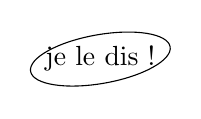
\begin{tikzpicture}[baseline=(t.base)]\node (t) {je le dis !};\draw[rotate=10] (0,0) ellipse (0.90 and 0.31);\end{tikzpicture}}}

\uline{pg48}\quad $\ell-4$\quad Pourquoi as-tu barré connexe ?

\deleted{\uline{pg53}\quad 5.7 est une redite pour $\ell\ne p$, et un peu idiot pour $\ell=p$.}\quad (utilisé en 5.15)

\figure{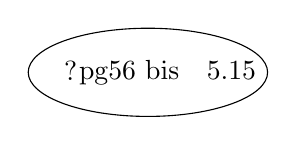
\begin{tikzpicture}[baseline=(t.base)]\node[inner sep=3pt] (t) {\uline{pg56 bis}\quad 5.15};\node at (-1.23,0.02) {?};\draw (-0.25,0) ellipse (1.52 and 0.56);\end{tikzpicture}}
tu n'a plus besoin ici de $\operatorname{car}(k)\ne\ell$

54 quater -- 5.11.\quad seraient plutôt que seront.

\uline{55 ter}\quad $\ell-10$. Il serait honnête de dire que 6.6 utilise $\operatorname{car}(K)=0$, via Tate
\margin{\figure{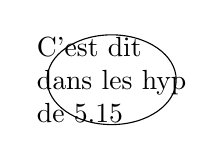
\begin{tikzpicture}[baseline=(t.base)]\node[align=left] (t) {C'est dit\\dans les \unsure{hyp}\\de 5.15};\draw (0,0) ellipse (0.82 and 0.57);\end{tikzpicture}}}

\figure{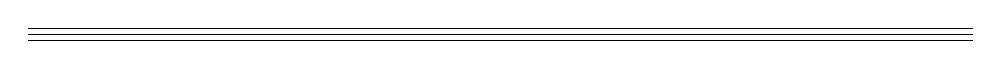
\begin{tikzpicture}\draw (0,0)--(12,0);\draw (0,-0.08)--(12,-0.08);\draw (0,-0.16)--(12,-0.16);\end{tikzpicture}}

\figure{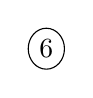
\begin{tikzpicture}[baseline=(t.base)]\node (t) {6};\draw (0,0) ellipse (0.23 and 0.26);\end{tikzpicture}}

\uline{pg57/58} : tu supposes tantôt $A^0$ $\ell$-divisible $(58,\ell-11)$, tantôt non $(57,\ell\,3)$

\uline{pg58}\quad $\ell-5$\quad
\figure{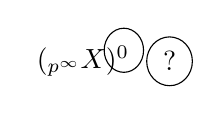
\begin{tikzpicture}[baseline=(t.base)]\node (t) {$( {}_{p^\infty}X)^0$};\draw (0.52,0.14) ellipse (0.25 and 0.28);\node at (1.10,0) {?};\draw (1.10,0) ellipse (0.29 and 0.31);\end{tikzpicture}}
\qquad itou plus loin --

\uline{pg59}\quad Je ne comprends rien -- Que fais-tu de la partie discrète ? --
\margin{\uline{CANULAR ?!}}

Je ne crois pas que la plus grande \deleted{\unsure{VA}} sous VA ordinaire puisse se relever (\unsure{$\hat{\mathrm m}$|ni} en cas de bonne réduction).

\uline{ie}\quad \unsure{6.3|63} est faux (déformer de façon générale $E\times F$, $E$ et $F$ elliptiques, $E$ ordinaire, $F$ non ordinaire ; général $\Rightarrow$ générique simple.

\margin{5}

\scanpage{7}
\mspage{5}
\margin{\figure{\begin{tikzpicture}\draw (0,0) .. controls (.1,-.2) and (.4,-.5) .. (.6,-.7);\end{tikzpicture}}}

\uline{pg60}\quad Je n'ai ps confiance en ``il est immédiat'' de 6.4.
\margin{\figure{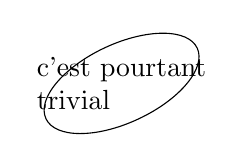
\begin{tikzpicture}[baseline=(t.base)]\node[align=left] (t) {c'est pourtant\\trivial};\draw[rotate=25] (0,0) ellipse (1.06 and 0.50);\end{tikzpicture}}}

\uline{pg61, 61 bis} : Je n'ai pas lu.

Il me semble qu'il doit être possible de définir, à isogénie près, des ``parties finies'' et ``parties toriques'', ayant le bon rang --
\margin{\figure{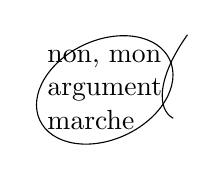
\begin{tikzpicture}[baseline=(t.base)]\node[align=left] (t) {non, mon\\argument\\marche};\draw[rotate=25] (0,0) ellipse (0.91 and 0.63);\draw (1.05,0.70) .. controls (0.66,0.15) and (0.66,-0.25) .. (0.87,-0.36);\end{tikzpicture}}}

\uline{pg\unsure{64|67}/\unsure{bis}} : \deleted{\unsure{voir}} (réf. à Serre pour \unsure{l'indép.|l'insép.} de $\ell$ ligne 11 ?)

Un peu malhonnête d'être si bref, car 6.6 est utilisé en 5.13.
\margin{\figure{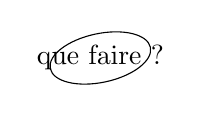
\begin{tikzpicture}[baseline=(t.base)]\node (t) {que faire ?};\draw[rotate=12] (0,0) ellipse (0.65 and 0.31);\end{tikzpicture}}}

\figure{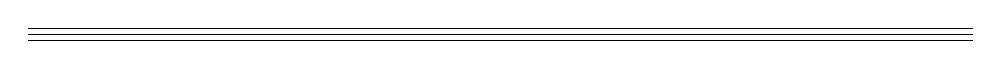
\begin{tikzpicture}\draw (0,0)--(12,0);\draw (0,-0.08)--(12,-0.08);\draw (0,-0.16)--(12,-0.16);\end{tikzpicture}}

\figure{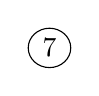
\begin{tikzpicture}[baseline=(t.base)]\node (t) {7};\draw (0,0) ellipse (0.27 and 0.25);\end{tikzpicture}}
\uline{p65}.\quad $A_0$ n'est pas défini\margin{si}

\uline{p.67}\quad (7.1.4)\quad français --
\margin{\figure{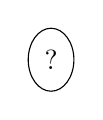
\begin{tikzpicture}[baseline=(t.base)]\node (t) {?};\draw (0,0) ellipse (0.29 and 0.40);\end{tikzpicture}}}

\figure{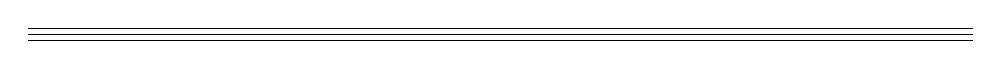
\begin{tikzpicture}\draw (0,0)--(12,0);\draw (0,-0.08)--(12,-0.08);\draw (0,-0.16)--(12,-0.16);\end{tikzpicture}}

\figure{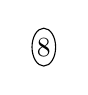
\begin{tikzpicture}[baseline=(t.base)]\node (t) {8};\draw (0,0) ellipse (0.15 and 0.24);\end{tikzpicture}}

\figure{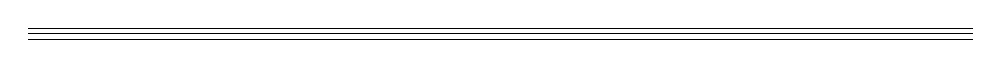
\begin{tikzpicture}\draw (0,0)--(12,0);\draw (0,-0.07)--(12,-0.07);\draw (0,-0.14)--(12,-0.14);\end{tikzpicture}}

\figure{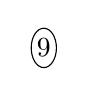
\begin{tikzpicture}[baseline=(t.base)]\node (t) {9};\draw (0,0) ellipse (0.16 and 0.25);\end{tikzpicture}}
\uline{p80}\quad 9.2.3\quad $u$ plutôt que $u(\unsure{g|q})$

\uline{p82}\quad (9.3.3)\quad $+$ compatibilité avec $R$ ? --

\uline{p87}\quad 9.4.\quad $S$ \uuline{strictement} hensélien ? (on le suppose en p88, $\ell-9$)

pas d'hyp. d'excellence ?

\uline{p91} : 9.5.8.\quad Ne mettrais-tu pas une génuflexion ``\unsure{au|en} signe près''.

\uline{pg92 bis}\quad $S$ est-il strictement hensélien ?

\figure{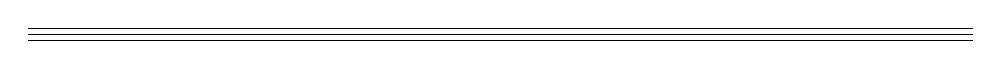
\begin{tikzpicture}\draw (0,0)--(12,0);\draw (0,-0.08)--(12,-0.08);\draw (0,-0.16)--(12,-0.16);\end{tikzpicture}}

\figure{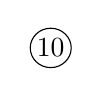
\begin{tikzpicture}[baseline=(t.base)]\node (t) {10};\draw (0,0) ellipse (0.26 and 0.25);\end{tikzpicture}}
\uline{pg98}\quad 10.5.3.\quad Une extension de $K$ (qui ici est infini) est-elle requise ??

10.5.4.\quad Dire \uline{où} on fera ces vérifications --

\margin{6}

\scanpage{8}
\mspage{6}
\margin{\figure{\begin{tikzpicture}\draw (0,0)--(.5,-.65);\end{tikzpicture}}}

\figure{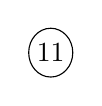
\begin{tikzpicture}[baseline=(t.base)]\node (t) {11};\draw (0,0) ellipse (0.28 and 0.31);\end{tikzpicture}}
pg101\quad $\ell-6$.\quad Dire où on trouve que Néron commute à $S\mapsto\widehat S$.

pg103\quad Le renvoi au courage du lecteur est désagréable --
\margin{\figure{\begin{tikzpicture}[baseline=(t.base)]\node (t) {que faire ?};\draw[rotate=12] (0,0) ellipse (0.96 and 0.41);\end{tikzpicture}}}

Si j'ai bien compris, tu affirme que prolonger une biextension à $A\times A'$ est ``la $\hat{\mathrm m}$ chose'' que de la prolonger aux ${}_{\ell^\infty}A\times{}_{\ell^\infty}A'$.

\margin{7}

\scanpage{28}

\diagram{\begin{tikzcd}[ampersand replacement=\&, row sep=small,column sep=small]
 \& M \arrow[dr,"{\text{\unsure{Situation}}}"] \& \& \& \unsure{-} \\
 \unsure{\bullet|0} \arrow[r,no head] \& T \arrow[r] \arrow[d,equal] \& G \arrow[r,no head] \& B \& 0 \arrow[l] \\
 \& D(M') \& \& \times \& \unsure{1|\vert} \\
 \unsure{\bullet|0} \arrow[r,no head] \& T' \arrow[r] \arrow[d,equal] \& G' \arrow[r,no head] \& B' \arrow[r] \& 0 \\
 \& D(M) \& \& \& \\
 \& M' \arrow[uur,"{\unsure{R^1}}"'] \& \& \&
\end{tikzcd}}

\margin{27}

\scanpage{29}

$\Gamma=\mathbb G$

\margin{$M\times B'\qquad\operatorname{Ext}(B',DM)$

$\deleted{\operatorname{Hom}(B',\operatorname{Ext}(\unsure{M},\unsure{\mathbb G_m}))}=0$}

\diagram{\begin{tikzcd}[ampersand replacement=\&, row sep=small,column sep=small]
B \& B'\\
M \arrow[u,"i"] \& M' \arrow[u,"i'"']
\end{tikzcd}}
\quad une biext.\inserted{$\mathcal E$} sous $\mathbb G_m$

\diagram{\begin{tikzcd}[ampersand replacement=\&, column sep=small]
B' \arrow[r,"\alpha'"] \& \underline{\operatorname{Ext}}(B,G_m) \arrow[r,no head] \& \underline{\operatorname{Ext}}(M,G_m)
\end{tikzcd}}
nul\quad p.c. $\operatorname{Hom}(B',\overset{\substack{0\\\Vert}}{\underline{\operatorname{Ext}}(M,G_m)}\unsure{)}$

\diagram{\begin{tikzcd}[ampersand replacement=\&, column sep=small]
B \arrow[r,no head,"\alpha"] \& \underline{\operatorname{Ext}}(B',G_m) \arrow[r,no head] \& \underline{\operatorname{Ext}}(M',G_m)
\end{tikzcd}}
nul\quad p.c. $\operatorname{Hom}(B,\underset{\substack{\Vert\\0}}{\underline{\operatorname{Ext}}(M',G_m)}\unsure{)}$

d'où extensions,

\diagram{\begin{tikzcd}[ampersand replacement=\&, column sep=small,row sep=tiny]
\unsure{\bullet|0} \arrow[r,no head] \& DM \arrow[r,"{\unsure{j'}}"] \arrow[d,equal] \& \unsure{G'|C'} \arrow[r,no head,"p'"] \& B' \arrow[r] \& 0\\
 \& T' \& \& \&
\end{tikzcd}}

\margin{\par\noindent\rule{0.8\linewidth}{0.3pt}\par
$\mathcal E_{M,G'}$ est \unsure{canoniqt} splitté par $\rho$
\par\noindent\rule{0.8\linewidth}{0.3pt}\par}

\diagram{\begin{tikzcd}[ampersand replacement=\&, column sep=small,row sep=tiny]
\unsure{\bullet|0} \arrow[r] \& DM' \arrow[r,no head,"{\unsure{j}}"] \arrow[d,equal] \& \unsure{G|C} \arrow[r,no head,"p"] \& B \arrow[r] \& 0\\
 \& T \& \& \&
\end{tikzcd}}

\margin{$\mathcal E_{G,M'}$ est can. splitté $\rho'$
\par\noindent\rule{0.8\linewidth}{0.3pt}\par}

\uline{\unsure{Exemple}} si \deleted{\unsure{par}} $\uline{\alpha'}$ \deleted{\unsure{était}} \inserted{\unsure{est}} un isom, alors $i'$ \unsure{revient à se donner}

un
\diagram{\begin{tikzcd}[ampersand replacement=\&, column sep=small]
i'\in\unsure{\operatorname{Hom}}(M',\underline{\operatorname{Ext}}(B,G_m)) \& \operatorname{Biext}(B,M';G_m) \arrow[l,"\sim"'] \& \deleted{\unsure{\operatorname{Hom}}}\inserted{\operatorname{Ext}(B,D(M'))} \arrow[l,"\sim"']
\end{tikzcd}}

\margin{si $\unsure{\operatorname{Ext}}(M',\underline{\operatorname{Hom}}(B,G_m))=0$

p.ex.
\figure{\begin{tikzpicture}[baseline=(t.base)]\node (t) {$\underline{\operatorname{Hom}}(B,G_m)=0$};\draw (0,0) ellipse (1.35 and 0.28);\end{tikzpicture}}}

\margin{si $\operatorname{Hom}(B,\underset{\substack{\Vert\\0}}{\underline{\operatorname{Ext}}(M',G_m)}\unsure{)}$ p.ex.
\figure{\begin{tikzpicture}[baseline=(t.base)]\node (t) {$\underline{\operatorname{Ext}}(M',G_m)=0$};\draw (0,0) ellipse (1.40 and 0.32);\end{tikzpicture}}}

\unsure{aussi} \unsure{pour}. Donc la donnée de $i'$ \unsure{équivaut à} celle de l'ext. $G$. Et réciproquement.

Considérons l'image inverse\inserted{\figure{\begin{tikzpicture}[baseline=(t.base)]\node (t) {$\mathcal E_{i,i'}$};\draw (0,0) ellipse (0.43 and 0.32);\end{tikzpicture}}}
de $\mathcal E$ sur $(M,M')$. Alors des \unsure{splittages}\inserted{$\unsure{\rho_i}$} de cette biextension correspondent aux hom $j$ de $M$ dans $G$ relevant $i$, \unsure{aux hom}\,$j'$ de $M'$ dans $G'$ relev. de $i'$.

\diagram{\begin{tikzcd}[ampersand replacement=\&, row sep=tiny,column sep=small]
M \arrow[r,no head] \& G \arrow[r,no head] \& B\\
M' \arrow[r,no head] \& G' \arrow[r,no head] \& B'
\end{tikzcd}}

\figure{\begin{tikzpicture}[baseline=(t.base)]\node (t) {\deleted{\unsure{sur $k$}}};\draw (0,0) ellipse (0.60 and 0.23);\end{tikzpicture}}

\inserted{Deux relèvements} \deleted{\unsure{si}} $j$ et $j'$ \deleted{\unsure{se}} \unsure{se correspondent ainsi},

\deleted{\unsure{Alors on trouve un} splitt. $\sigma$ canonique \deleted{$\unsure{\sigma'}$} de $\mathcal E_{G,M'}$ et un splitt. $\sigma'$ canonique de $\mathcal E_{M,G'}$, ces deux splittages coïncident sur $M,M'$ avec le splittage \unsure{donné} $h$ de $\mathcal E_{M,M'}$.}

ssi les deux splittages de $\mathcal E_{M,M'}$, déduits d'une part du splittage $\rho$ de $\mathcal E_{M,G'}$ \unsure{et de} $j':M'\longrightarrow G'$, d'autre part du splittage $\rho'$ de $\mathcal E_{G,M'}$ et de $j:M\mathbin{-}G$, coïncident.

\margin{28}

\scanpage{30}

or le premier membre (grâce à (2.3.2)) est $\phi^{n'}(x,my)=m\phi^{n'}(x,y)$. La compatibilité \deleted{(2.3.1)} (\unsure{2.3.2|2.2.2}) \deleted{est}\inserted{implique} à son tour \deleted{\unsure{conséquence de}} la compatibilité symétrique\inserted{de (2.3.1)}, exprimée par la commutativité de

(2.3.\unsure{4|3})
\diagram{\begin{tikzcd}[ampersand replacement=\&, column sep=small,row sep=large]
\deleted{\unsure{et}} \& {}_nP \arrow[d,"\mathrm{id}"'] \& \times \& {}_{n'}Q \arrow[d,"m"] \arrow[rr,"{\phi^{n'}_\xi|_{{}_nP\times{}_{n'}Q}}"] \& \& {}_nG \arrow[d,"\mathrm{id}"]\\
 \& {}_nP \& \times \& {}_nQ \arrow[rr,"\phi^n_\xi"] \& \& {}_nG
\end{tikzcd}},

qui s'écrit en formules
\[
(2.3.\unsure{5|4})\qquad \phi^n(x,my)=\phi^{n'}(x,y)\qquad (x\in{}_nP(S),\ y\in{}_nQ(S)).
\]

\deleted{Montrons comment (2.3.\unsure{2}) implique (2.3.\unsure{4}), avec les notations de cette dernière formule,}
Comme ${}_{mn'}P\xrightarrow{m}{}_nP$ est un épimorphisme, on est ramené à prouver (2.3.2) dans le cas où $x=mx'$, où $x'\in{}_{n'}P(S)$, \deleted{donc}\inserted{or} on a
\[
\deleted{\unsure{\phi^n(mx,y)=\phi^n(m^2x',y)=\phi^n}}
\quad
\phi^n_{\inserted{\xi}}(mx',my)\overset{\inserted{(2.3.3)}}{=}m\phi^{n'}_{\inserted{\xi}}(x',y)=\phi^{n'}_{\inserted{\xi}}(mx',y)
\]
(par bilinéarité de $\phi^{n'}$) $=\phi^{n'}_{\inserted{\xi}}(x,y)$ puisque $x=mx'$ dans ${}_{n'}P(S)$, ce qui établit (2.3.5).

Prouvons donc la compatibilité (2.3.1). La fonctorialité\inserted{en $Q$} de l'\unsure{hmomorphisme|homomorphisme} (2.1.2) nous montre qu'on peut supposer $nQ=0$. Alors (2.1.2) est le composé

\diagram{\begin{tikzcd}[ampersand replacement=\&, column sep=small]
\operatorname{Biext}^1(P,Q;G) \arrow[r,"\sim"] \& \operatorname{Hom}(\underline{\operatorname{Tor}}_1(P,Q),G) \& \operatorname{Hom}({}_nP\otimes Q,G) \arrow[l,"\sim"']
\end{tikzcd}},

\deleted{en $Q$ nous montre que (2.1.2) est le composé}
\[
\deleted{\operatorname{Biext}^1(P,Q;G)\qquad\operatorname{Hom}(\operatorname{Tor}_1(P,Q),G)\qquad\operatorname{Hom}(\operatorname{Tor}_1(P,{}_nQ),G)}
\]

où la première flèche est celle de (1.1.3) et ne dépend pas du choix de $n$, et où la deuxième flèche est transposée de l'isomorphisme $\underline{\operatorname{Tor}}_1(P,Q)\overset{\inserted{\unsure{\delta|\partial}}}{\xrightarrow{\sim}}{}_nP\otimes Q$ défini dans (1.3.4). Donc la compatibilité voulue équivaut essentiellement à \deleted{\unsure{voir}} la commutativité du diagramme

\diagram{\begin{tikzcd}[ampersand replacement=\&, row sep=small,column sep=large]
 \& {}_{n'}P\otimes Q \arrow[dd,"m\otimes\mathrm{id}_Q"]\\
\underline{\operatorname{Tor}}_1(P,Q) \arrow[ur] \arrow[dr] \& \\
 \& {}_nP\otimes Q\quad\deleted{\unsure{+}}\quad\deleted{\unsure{\xi}}
\end{tikzcd}},

où les flèches obliques sont les deux isomorphismes du type (1.3.4), relatifs à $n$ et $n'$ respectivement. Or cette compatibilité résulte de

\margin{29}

\scanpage{31}

Supposons $j$ et $j'$ ainsi \unsure{choisis}. Si $j,j'$ sont injectifs, on en déduit une biextension \inserted{\figure{\begin{tikzpicture}[baseline=(t.base)]\node (t) {canonique};\draw (0,0) ellipse (.8 and .22);\end{tikzpicture}}} de $(A,A')$, où $A=G/M$, $A'=G'/M'$. Dans le cas général, posons

\deleted{pour dire qu'on a une biextension de}
\[
A=\left[\underset{\text{deg.}\,-1}{M}\longrightarrow\underset{\text{deg}\,0}{G}\right]\ ;\qquad
A'=\left[M'\mathbin{-}G'\right].
\]

d'où
\diagram{\begin{tikzcd}[ampersand replacement=\&, row sep=small,column sep=small]
 \& \& A \arrow[dl,"1"'] \& \& \& \& A' \arrow[dl,"1"'] \& \\
\phantom{0} \& M \arrow[l,no head] \arrow[r] \& G \arrow[u] \arrow[r,no head] \& \phantom{0} \& \text{\unsure{cônes de morphismes}} \& M' \arrow[l,no head] \& G' \arrow[u] \arrow[l,no head] \&
\end{tikzcd}}

on va définir une \deleted{\unsure{biextension}} classe canonique
\[
\xi\in\operatorname{Ext}^1(A\mathbin{\overset{L}{\otimes}}A',G_m),
\]
jouant le rôle d'une biextension de $(A,A')$ par $G_m$.

Soit en effet \figure{\begin{tikzpicture}[baseline]\draw(0,.08)--(.1,.04);\draw(.16,.04)--(.26,.04);\draw(.31,.03)--(.43,.06);\draw(.53,.04)--(.82,.07);\draw(.94,.04)--(1.06,.08);\end{tikzpicture}}
\margin{\unsure{pourquoi ?}}
\figure{\begin{tikzpicture}\draw (0,2.4) .. controls (-.18,1.6) and (-.2,.5) .. (0,.25) .. controls (.2,.05) and (.17,-.12) .. (.06,-.2);\end{tikzpicture}}

\unsure{Soit}
\[
{}_nA\overset{\text{déf}}{=}\deleted{\unsure{R}}\underline{\operatorname{Ext}}^0(\unsure{\mathbb Z|\mathbf Z}/n\unsure{\mathbb Z|\mathbf Z},A),\qquad
{}_nA'=\underline{\operatorname{Ext}}^0(\unsure{\mathbb Z|\mathbf Z}/n\unsure{\mathbb Z|\mathbf Z},A')
\]
on trouve, \unsure{grâce, par} aux triangles plus haut,
\margin{\deleted{\uline{\unsure{et}}}}
\[
\left\{\begin{aligned}
{}_nM&=0\quad\deleted{\unsure{{}_nM'=0}}\quad\inserted{\figure{\begin{tikzpicture}[baseline=(t.base)]\node (t) {\unsure{resp.}};\draw (0,0) circle (.35);\end{tikzpicture}}}\\
nG&=G\quad\text{puisque}\quad\deleted{\unsure{par}}\ nB=B,\ nT=T\quad(\text{ce dernier résulte de }{}_n\unsure{M|M'}=0
\end{aligned}\right.
\]

\margin{donne aussi autre \unsure{interprét\textsuperscript{tion}} de ${}_nA$, via hom. cobord si $nG=G$}
\figure{\begin{tikzpicture}\draw (0,0)--(0,1.7);\end{tikzpicture}}
\diagram{\begin{tikzcd}[ampersand replacement=\&, column sep=small]
0 \arrow[r] \& \underset{\underbrace{\vphantom{G}}_{(D(M'_n),{}_nB),\ \text{si }nT=T}}{ {}_nG} \arrow[r] \& {}_nA \arrow[r] \& M_n \arrow[r] \& 0
\end{tikzcd}}

et \unsure{on a de $\widehat{\mathrm m}$} une suite exacte
\diagram{\begin{tikzcd}[ampersand replacement=\&, column sep=small]
0 \arrow[r] \& {}_nG' \arrow[r] \& {}_nA' \arrow[r] \& M'_n \arrow[r] \& 0
\end{tikzcd}}

sous les hyp. duales; passant à la limite sur $n=\ell^\nu$, on a
\[
\left\{\begin{gathered}
\diagram{\begin{tikzcd}[ampersand replacement=\&, column sep=small]0 \arrow[r] \& T_\ell(\unsure{G}) \arrow[r,no head] \& T_\ell(A) \arrow[r] \& M\otimes\unsure{\mathbb Z|\mathbf Z}_\ell \arrow[r,no head] \& 0\end{tikzcd}}\\
\diagram{\begin{tikzcd}[ampersand replacement=\&, column sep=small]0 \arrow[r,no head] \& T_\ell(\unsure{A'|G'}) \arrow[r,no head] \& T_\ell(A') \arrow[r,no head] \& M'\otimes\unsure{\mathbb Z|\mathbf Z}_\ell \arrow[r] \& 0\end{tikzcd}}
\end{gathered}\right.
\]
\margin{30}

\scanpage{32}

\margin{\figure{\begin{tikzpicture}\node (a) at (0,.3) {$\phi^{(\ell)}$};\node (b) at (.35,-.45) {${}_{\ell^\nu}P$};\draw[rotate=20] (0,.3) ellipse (.45 and .65);\draw[rotate=20] (.35,-.45) ellipse (.43 and .55);\end{tikzpicture}}}
\[
(2.2.4)\qquad\deleted{\unsure{\$}}\phi^{(\ell)}_\xi\deleted{\unsure{\$}}=(\phi^{\ell^\nu}_\xi)_{\nu\geq0},\quad\text{où}\quad\phi^{\ell^\nu}_\xi:{}_{\ell^\nu}P\times{}_{\ell^\nu}Q\longrightarrow G.
\]
Les diagrammes \deleted{déduits}\inserted{commutatifs} de (2.2.2) en y faisant $n=\ell^\nu$, $n'=\ell^{\nu'}$, pour $\nu'\geq\nu$, montrent que $\phi^{(\ell)}_\xi$ peut être interprété comme un accouplement de \deleted{\unsure{progroupes}} systèmes projectifs de groupes
\[
(2.2.5)\qquad\phi^{(\ell)}_\xi:T_\ell(P)\times T_\ell(Q)\longrightarrow T_\ell(G),
\]
où, pour un groupe $M$ de $T$ et un nombre premier $\ell$, on désigne par
\[
T_\ell(M)=({}_{\ell^\nu}M)_{\nu\geq0}
\]
le système projectif des ${}_{\ell^\nu}M$. L'accouplement \deleted{\unsure{\$}} (2.2.5) est encore appelé \uline{l'accouplement} $\ell$\uline{-adique associé à} $\xi$ (ou à la biextension $E$ de classe $\xi$). Pour $\xi$ variable, on obtient un homomorphisme canonique
\[
(2.2.6)\qquad\operatorname{Biext}^{\inserted{1}}(P,Q;G)\longrightarrow\operatorname{Hom}(T_\ell(P)\otimes T_\ell(Q),T_\ell(G)).
\]
On notera que les homomorphismes (2.1.2) sont \uline{fonctoriels} en $P,Q,G$ (pour $n$ fixé), d'où on déduit qu'il en est de même de (2.2.6).

\figure{\begin{tikzpicture}\draw (0,0)--(1.7,.07);\draw (-.1,-.13)--(1.85,-.1);\end{tikzpicture}}

2.3. \deleted{On peut regarder} La compatibilité (2.2.2) permet de retrouver $\phi^n_\xi$ connaissant $\phi^{n'}_\xi$, pourvu que ${}_{n'}Q\xrightarrow{m}{}_nQ$ \inserted{soit} un épimorphisme, --- \deleted{\unsure{(NB la}} condition satisfaite, comme il est bien connu, si $nQ=Q$. En effet, comme ${}_{n'}P\xrightarrow{m}{}_nP$ est aussi un épimorphisme, $\phi^n_\xi$ se déduit alors de $\phi^{n'}_\xi$ par passage au quotient. On peut cependant \inserted{donner} une compatibilité légèrement plus précise que (2.2.2), qui permet d\deleted{\unsure{e}}'exprimer $\phi^n$ en termes de $\phi^{n'}$ sans aucune restriction sur $Q$, par la commutativité de

(2.3.1)
\diagram{\begin{tikzcd}[ampersand replacement=\&, column sep=small,row sep=large]
{}_{n'}P \arrow[d,"m"'] \& \times \& {}_nQ \arrow[d,"\mathrm{id}"] \arrow[rr,"{\phi^{n'}_\xi|_{{}_{n'}P\times{}_nQ}}"] \& \& {}_nG \arrow[d,"\mathrm{id}"]\\
{}_{\deleted{\unsure{m}}n}P \& \times \& {}_nQ \arrow[rr,"\phi^n_\xi"] \& \& {}_nG
\end{tikzcd}},

en formules
\[
(2.3.2)\qquad\phi^n_\xi(mx,y)=\phi^{n'}_\xi(x,y)\qquad(x\in{}_{n'}P(S),\ y\in{}_nQ(S)).
\]
Cette formule implique évidemment la commutativité de (2.2.2), qui s'écrit en effet
\[
\inserted{(2.3.3)}\qquad\phi^n_\xi(mx,my)=m\phi^{n'}_\xi(x,y)\qquad(x\in{}_{n'}P(S),\ y\in{}_{n'}P(S)),
\]
\margin{31}

\scanpage{33}

\deleted{\unsure{Les inclusions}}

on a \uline{loc.} des hom
\[
{}_nA\longrightarrow A,\qquad{}_nA'\longrightarrow A'.
\]
d'où \uline{loc.} \unsure{un hom.}
\diagram{\begin{tikzcd}[ampersand replacement=\&, column sep=large,row sep=large]
\operatorname{Ext}^1(A\mathbin{\overset{L}{\otimes}}A\unsure{'},G_m) \arrow[r] \arrow[dr] \& \operatorname{Ext}^1({}_nA\mathbin{\overset{L}{\otimes}}{}_nA',G_m)\unsure{\to0} \arrow[d]\\
 \& \operatorname{Hom}({}_nA\otimes{}_nA',G_m)
\end{tikzcd}}

\unsure{qui se recollent}, donc \unsure{un hom défini global\textsuperscript{t}}. Donc l'élément $\xi$ envisagé plus haut nous donne
\[
\phi_n^\xi:{}_nA\otimes{}_nA'\longrightarrow G_m
\]
et par passage à la limite
\[
T_\ell(A)\times T_\ell(A')\longrightarrow T_\ell G_m)\overset{\text{déf}}{=}\unsure{\mathbb Z|\mathbf Z}_\ell(1).
\]

\uline{\unsure{Prop.|Rmq}} Dans cet accouplement, $D(\unsure{M'_n|M_n})$ est orthogonal à ${}_nG'$, \deleted{\unsure{et}} (a un sens si ${}_nM'=0$) et \deleted{$\unsure{D(M_n)}$} ${}_nG$ est orth. à $D(M_n)$ (a un sens si ${}_nM=0$). Les accouplements induits
\figure{\begin{tikzpicture}\draw (0,0)--(0,1.8);\end{tikzpicture}}

\diagram{\begin{tikzcd}[ampersand replacement=\&, column sep=small,row sep=small]
\deleted{\unsure{{}_nA/}} \& {}_nA'/{}_nG' \& \times \& D(M'_n) \arrow[rr] \arrow[ll,bend right=75,no head] \& \& G_m\\
 \& \wr \& \& \Vert \& \&\\
 \& M'_n \& \& {}_nT \& \&
\end{tikzcd}}

et
\diagram{\begin{tikzcd}[ampersand replacement=\&, column sep=small,row sep=small]
D(M_n) \& \times \& \unsure{{}_nA|A}/{}_nG \arrow[r,no head] \& G_m\\
\Vert \& \& \wr \&\\
{}_nT \& \& M_n \&
\end{tikzcd}},

ainsi que
\diagram{\begin{tikzcd}[ampersand replacement=\&, column sep=small,row sep=small]
\deleted{\unsure{et}} \& {}_nG/{}_nT \& \times \& {}_nG'/{}_nT'\\
 \& \Vert\ \deleted{\unsure{\text{et}}} \& \& \wr\\
 \& {}_nB \& \& {}_nB'
\end{tikzcd}}
sont ceux qu'on devine.

\uline{Corollaire} Si l'accouplement entre ${}_nB$ et ${}_nB'$ est une dualité parfaite (car $\unsure{{}_nT_n}=\unsure{{}_nT'_n}=0$) \deleted{\unsure{donc}} et si ${}_nM=0$, ${}_nM'=0$, $nB=B$, $nB'=B'$, alors l'accouplement de ${}_nA$ et ${}_nA'$ est une dualité parfaite.
\figure{\begin{tikzpicture}\draw (0,0)--(0,2);\end{tikzpicture}}
\margin{32}

\scanpage{34}

2. \uline{Accouplements définis par une biextension}.

2.1. Soit $n$ un entier $>0$, et supposons qu'on a
\[
(2.1.1)\qquad nP=P.
\]
Considérons alors l'homomorphisme composé
\figure{\begin{tikzpicture}\draw (0,0)--(1.5,.08);\draw (.08,-.1)--(1.3,-.05);\end{tikzpicture}}

(2.1.2)
\diagram{\begin{tikzcd}[ampersand replacement=\&, column sep=large]
\operatorname{Biext}^{\inserted{1}}(P,Q;G) \arrow[r] \arrow[rr,bend left=20,"\phi^n"] \& \operatorname{Biext}^{\inserted{1}}(P,{}_nQ;G) \arrow[r,"\sim"] \& \operatorname{Hom}({}_nP\otimes{}_nQ;G)
\end{tikzcd}},

où la première flèche est la restriction à $(P,{}_nQ)$, et la deuxième est l'isomorphisme (1.3.6). Il permet, à tout élément \figure{\begin{tikzpicture}[baseline=(x.base)]\node(x){$\xi\in\operatorname{Biext}(P,Q;G)$};\draw(0,0)ellipse(1.9 and .4);\draw[->](-1.9,-.2)..controls(-2.2,-.4)and(-3.7,-.2)..(-4.1,-.45);\end{tikzpicture}},

(2.1.3)

à fortiori à toute biextension \inserted{\figure{\begin{tikzpicture}[baseline=(e.base)]\node(e){$E$};\draw(0,0)ellipse(.27 and .22);\draw(.17,-.18)--(0,-.45);\end{tikzpicture}}} de $(P,Q)$ par $G$, de faire correspondre un\deleted{e \unsure{forme homomorphisme}} accouplement bilinéaire
\margin{\figure{\begin{tikzpicture}\node at(0,0){$\phi$};\draw[rotate=15](0,0)ellipse(.35 and .5);\end{tikzpicture}}}
\[
(2.1.4)\qquad\phi_\xi\text{ ou }\phi^n_\xi:{}_nP\times{}_nQ\longrightarrow G,
\]
qu'on appelle l'accouplement \uline{associé à} $\xi$ (ou à la biextension $E$).

2.2. Soit \deleted{\unsure{n}} $n'$ un multiple de $n$,
\[
n'=mn,
\]
et supposons qu'on ait la relation (plus forte que (2.1.1))
\[
(2.2.1)\qquad n'P=P\quad\text{i.e.}\quad mnP=P,
\]
d'où comme en (2.1.4), pour toute $\xi\in\operatorname{Biext}(P,Q;G)$, un\deleted{e} accouplement
\[
\phi^{n'}_\xi:{}_{n'}P\times{}_{n'}Q\longrightarrow G.
\]
\deleted{Les relations entre cet accouplement et}\inserted{Il est lié à} l'accouplement $\phi^n_\xi$ \deleted{est donné} par la commutativité du diagramme suivant (\deleted{qu'on laisse au lecteur le soin d'établir)}\inserted{cf. 2.3 ci-dessous pour une démonstration)}:

(2.2.2)
\diagram{\begin{tikzcd}[ampersand replacement=\&, column sep=small,row sep=large]
{}_{n'}P \arrow[d,"m"'] \& \times \& {}_{n'\deleted{\unsure{n}}}Q\deleted{\unsure{Q}} \arrow[d,"m"] \arrow[rr,"\phi^{n'}_\xi"] \& \& {}_{n'}G \arrow[d,"m"]\\
\deleted{\unsure{P}}{}_nP \& \deleted{\unsure{\times}}\times \& {}_nQ \arrow[rr,"\phi^n_\xi"] \& \& {}_nG
\end{tikzcd}},
\inserted{où les flèches verticales sont induites par la multiplication par $m=n'/n$.}

Notons maintenant que moyennant (2.1.1), on peut prendre pour $n'$ n'importe quelle puissance de $n$. En particulier, soit \figure{\begin{tikzpicture}[baseline=(l.base)]\node(l){$\ell$};\draw[rotate=-10](0,0)ellipse(.22 and .5);\end{tikzpicture}} un nombre premier, et supposons que\deleted{\unsure{e}} l'on ait
\margin{\figure{\begin{tikzpicture}\node at(0,0){$\ell$};\draw[rotate=-20](0,0)ellipse(.3 and .5);\end{tikzpicture}}}
\[
(2.2.3)\qquad\figure{\begin{tikzpicture}[baseline=(l.base)]\node(l){$\ell$};\draw[rotate=-20](0,0)ellipse(.23 and .55);\end{tikzpicture}} P=P,
\]
et considérons le système des accouplements
\margin{33}

\scanpage{35}
\uline{Picard et dualité}
\margin{34}

\scanpage{36}
\figure{\begin{tikzpicture}[baseline=(t.base)]
\node[inner sep=0pt] (t) {\diagram{\begin{array}{l|l|l}
\begin{gathered}
H^0(X,\zeta_\ell)=\unsure{U_\ell|\mu_\ell}\\[1em]
\begin{aligned}
H^2(X,\mathbb Z/\ell)&=H^2(X,\zeta_\ell)\otimes_{\mathbb Z/\ell}\operatorname{Hom}(U_\ell,\mathbb Z/\ell)\\
&=\unsure{\mathbb Z_\ell|\mathbb Z/\ell}\otimes_{\mathbb Z/\ell}\operatorname{Hom}(U_\ell,\mathbb Z/\ell)\\
&\simeq\deleted{\unsure{\mathbb Z/\ell}}\operatorname{Hom}(U_\ell,\mathbb Z/\ell)
\end{aligned}
\end{gathered}
&
\begin{gathered}
H^1(X,\zeta_\ell)=P^{(\ell)}\quad\text{\unsure{Points} de la jacobienne}\\
\text{$P$ de $X$, annulés par $\ell$}\\[1em]
\begin{aligned}
H^1(X,\mathbb Z/\ell)&=H^1(X,\zeta_\ell)\otimes_{\mathbb Z/\ell}\operatorname{Hom}(\unsure{U_\ell},\mathbb Z/\ell)\\
&\deleted{=P^{(\ell)}\mathbin{\underset{\text{''}}{\otimes}}\operatorname{Hom}(\zeta_\ell,\unsure{H})}\\
&=P^{(\ell)}\otimes_{\mathbb Z/\ell}\operatorname{Hom}(\unsure{U_\ell},\mathbb Z/\ell)
\end{aligned}\\[1em]
\text{Or}\quad P^{(\ell)}\times P^{(\ell)}\longrightarrow U_\ell\quad\text{\unsure{en vertu}}\\
\text{de}\quad\boxed{\begin{gathered}\text{l'autodualité de }P\ \mathbin{-}\mathbin{-}\\\text{et la dualité de Kummer-Serre}\end{gathered}}
\end{gathered}
&
\begin{gathered}H^2(X,\zeta_\ell)\simeq\mathbb Z/\ell\\[2em]H^0(X,\mathbb Z/\ell)\simeq\mathbb Z/\ell\end{gathered}
\\\hline
\begin{gathered}H^0(X,\zeta_p)=0\\[1.5em]H^2(X,\mathbb Z/p)\simeq H^2(X,\mathbb Z/p)=0\end{gathered}
&
\begin{gathered}
H^1(X,\zeta_p)=P^{(p)}:\ \text{\unsure{élts} d'ordre $p$}\\
\text{de la jacobienne}\\[1em]
H^1(X,\mathbb Z/p)\simeq\text{\unsure{Points} de }H^1(X,\underline{\mathrm O}_X)\text{ fixes}\\
\text{par }F\\
\boxed{\text{dualité de Serre - Cartier}}
\end{gathered}
&\begin{gathered}H^2(X,\zeta_p)\simeq\mathbb Z/p\\[2em]H^0(X,\mathbb Z/p)\simeq\mathbb Z/p\end{gathered}
\\\hline
H^0(X,\unsure{i_p|\alpha_p})=0
& H^1(X,\unsure{i_p})\simeq{}_{F}H^1(X,\underline{\mathrm O}_X)\deleted{\unsure{F}}
& H^2(X,\unsure{i_p})=H^1(X,\underline{\mathrm O}_X)_F
\end{array}}};
\coordinate (a) at ($(t.north west)!.07!(t.south west)$);
\coordinate (b) at ($(t.north west)!.60!(t.south west)$);
\coordinate (c) at ($(t.north west)!.95!(t.south west)$);
\draw ([xshift=-3mm]a) .. controls ([xshift=-7mm]a) and ([xshift=-4mm,yshift=9mm]b) .. ([xshift=-5mm,yshift=2mm]b)
.. controls ([xshift=-6mm]b) and ([xshift=-7mm]b) .. ([xshift=-9mm]b)
.. controls ([xshift=-2mm]b) and ([xshift=-7mm,yshift=4mm]c) .. ([xshift=-3mm]c);
\node[rotate=90,anchor=south] at ([xshift=-11mm,yshift=7mm]b) {\begin{minipage}{5cm}\margin{Cohomologie discrète}\end{minipage}};
\node[anchor=east] at ([xshift=-10mm,yshift=-5mm]b) {\begin{minipage}{8mm}\margin{$*$\unsure{[}}\end{minipage}};
\end{tikzpicture}}
\margin{35}

\scanpage{37}
\[
H^1\bigl(X,\underbrace{\underline{\operatorname{Ext}}^1(f^*(B),G_{mX})}\bigr)
\]
\margin{\unsure{.\ '}}
\diagram{\begin{tikzcd}[ampersand replacement=\&, column sep=large,row sep=large]
\operatorname{Ext}_X(\overbrace{f^*(B)}^{A},G_{mX})\simeq\operatorname{Ext}_S(B,f_!(G_{mX}))\\
H^p(X,\underline{\operatorname{Ext}}^q_X(A,G_{mX})) \arrow[u,Rightarrow]
\end{tikzcd}}

\figure{\begin{tikzpicture}\draw (0,.05)--(10,0);\end{tikzpicture}}

Suite exacte de Cohomologie. Critère de \unsure{surjectivité};

\unsure{Fibré universel}

Dualité de Cartier [voir \unsure{Pic.}\ldots]

Th. \unsure{projectivité} des V.A. (Th. de rigidité)

Propriétés \unsure{finicielles|fonctorielles} des groupes \ldots

Propriétés différentielles des \unsure{gpes} et fibrés

En particulier : \uuline{fibrés linéaires}, symplectiques, orthogonaux etc \ldots

\figure{\begin{tikzpicture}\draw (0,3.6) .. controls (-.14,3.7) and (-.08,2.9) .. (-.1,2.6) .. controls (-.18,2.4) and (-.26,2.8) .. (-.14,2.5) .. controls (.1,1.7) and (-.1,.3) .. (.35,0);\draw (.05,1.3)--(.22,1.05);\end{tikzpicture}}

\unsure{Leur dualité} \unsure{pour} les \unsure{représentations lin. de groupes} ??

\figure{\begin{tikzpicture}\draw (0,0)--(10,.05);\end{tikzpicture}}
\[
\deleted{\underline{\operatorname{Hom}}(G_a,G_m)}
\]
\[
\mathbb Z.\quad\unsure{\vdash|\mapsto}\quad\mathbb Z
\]
\margin{36}

\scanpage{38}

\begin{center}-- 98 --\end{center}
\margin{n\textsuperscript{o} 316}

un automorphisme de $E$.

Si en outre $E$ est une algèbre (non nécessairement associative), et si $u$ est une dérivation (nilpotente) de $E$, alors $e^u$ est un automorphisme de \uline{l'algèbre} $E$. En effet, si $x,y\in E$, on a
\[
u^p(xy)=\sum_{r+s=p}\binom{p}{r}u^r(x)u^s(y)
\]
pour tout entier $p\geq0$ (formule de Leibniz). Il en résulte que :
\[
\begin{aligned}
e^u(xy)&=\sum_{p\geq0}\frac{1}{p!}u^p(xy)=\sum_{p\geq0}\sum_{r+s=p}\frac{u^r(x)}{r!}\frac{u^s(y)}{s!}\\
&=\sum_{r,s=0}^\infty\frac{u^r(x)}{r!}\frac{u^s(y)}{s!}=e^u(x)e^u(y)
\end{aligned}
\]
d'où notre assertion.

Soit maintenant $\mathfrak g$ une algèbre de Lie. Si $x$ appartient au radical nilpotent de $\mathfrak g$, la dérivation $\operatorname{ad}_{\mathfrak g}x$ de $\mathfrak g$ est nilpotente. On peut donc poser la définition suivante :

\uline{Définition} 5 -- \uline{On appelle automorphisme spécial de} $\mathfrak g$ \uline{un automorphisme de} $\mathfrak g$ \uline{de la forme} $e^{\operatorname{ad}x}$, \uline{où} $x$ \uline{est dans le radical nilpotent de} $\mathfrak g$.

Il est clair qu'un automorphisme spécial laisse stable tout idéal de $\mathfrak g$.

\uline{Définition} 6 -- \uline{Soient} $\mathfrak g$ \uline{une algèbre de Lie}, $\unsure{\mathfrak r|r}$ \uline{son radical}. \uline{On appelle sous-algèbre de Levi de} $\mathfrak g$ \uline{toute sous-algèbre supplémentaire de} $\unsure{\mathfrak r|r}$ \uline{dans} $\mathfrak g$.

Une sous-algèbre de Levi est isomorphe à $\mathfrak g/\unsure{\mathfrak r|r}$, donc semi-simple. Comme une sous-algèbre semi-simple n'a que $0$ en commun avec $\unsure{\mathfrak r|r}$, toute sous-algèbre semi-simple $\unsure{\mathfrak h|h}$ telle que $\mathfrak g=\unsure{\mathfrak r|r}+\unsure{\mathfrak h|h}$ est une sous-algèbre de Levi ; par conséquent, l'image d'une sous-algèbre de Levi par un homomorphisme surjectif est une sous-algèbre de Levi.
\margin{37}

\scanpage{39}

$X$ propre et simple sur $k$ [\unsure{généralisons|généralisable} à une base quelconque]

$A$ V.A. sur $k$

$H^1(X,A)=\underset{n}{\varinjlim}\ {}_nH^1(X,A)$ \deleted{$\unsure{=}$} d'autre part on a une suite exacte
\diagram{\begin{tikzcd}[ampersand replacement=\&, column sep=small]
0 \arrow[r] \& \operatorname{Hom}(X,A)_n \arrow[r] \& \deleted{\unsure{n}}H^1(X,{}_nA) \arrow[r] \& {}_nH^1(X,A) \arrow[r] \& 0
\end{tikzcd}}
qui s'écrit aussi
\diagram{\begin{tikzcd}[ampersand replacement=\&, column sep=small]
0 \arrow[r] \& \operatorname{Hom}(\operatorname{Alb}_X,A)_n \arrow[r] \& \operatorname{Hom}(D({}_nA),\operatorname{Pic}_X) \arrow[r] \& {}_nH^1(X,A) \arrow[r] \& 0
\end{tikzcd}}

ou encore, sachant que
\[
\operatorname{Hom}(\operatorname{Alb}_X,A)\simeq\operatorname{Hom}(A',(\operatorname{Alb}_X)')=\operatorname{Hom}(A',\operatorname{Pic}_X^0)
\]
\[
D({}_nA)\simeq{}_nA'
\]
une suite exacte

$(*)$
\diagram{\begin{tikzcd}[ampersand replacement=\&, column sep=small]
0 \arrow[r] \& \operatorname{Hom}(A',\operatorname{Pic}_X^{\unsure{0}})_n \arrow[r] \& \operatorname{Hom}({}_nA',\operatorname{Pic}_X) \arrow[r] \& {}_nH^1(X,A) \arrow[r] \& 0
\end{tikzcd}}
et passant à la limite \inserted{\unsure{inductive}} on a :
\diagram{\boxed{\begin{tikzcd}[ampersand replacement=\&, column sep=small]
0 \arrow[r] \& \operatorname{Hom}(A',\underline{\operatorname{Pic}}_X^0)\otimes_{\mathbb Z}\mathbb Q \arrow[r] \& \operatorname{Hom}(T_{\unsure{\cdot}}(A'),\underline{\operatorname{Pic}}_X) \arrow[r,no head] \& H^1(X,A) \arrow[r] \& 0
\end{tikzcd}}}

Or la suite exacte $(*)$ se compare à la suite exacte déduite de
\diagram{\begin{tikzcd}[ampersand replacement=\&, column sep=small]
0 \arrow[r,no head] \& {}_nA' \arrow[r,no head] \& A' \arrow[r] \& A' \arrow[r] \& 0
\end{tikzcd}}
en appliquant $\deleted{\operatorname{Ext}}\underline{\operatorname{Hom}}(-,\operatorname{Pic}_X)$, on \unsure{trouve}

$(**)$
\diagram{\begin{tikzcd}[ampersand replacement=\&, column sep=small]
0 \arrow[r,no head] \& \operatorname{Hom}(A',\underline{\operatorname{Pic}}_X)_n \arrow[r] \& \operatorname{Hom}({}_nA',\underline{\operatorname{Pic}}_X) \arrow[r] \& {}_n\operatorname{Ext}^1(A',\underline{\operatorname{Pic}}_X^{\unsure{\tau|2}}) \arrow[r] \& 0
\end{tikzcd}}
qui donne à la limite
\diagram{\boxed{\begin{tikzcd}[ampersand replacement=\&, column sep=small,row sep=tiny]
0 \arrow[r,no head] \& \operatorname{Hom}(A',\operatorname{Pic}_X)\otimes_{\mathbb Z}\mathbb Q \arrow[r] \& \operatorname{Hom}(T_{\unsure{\cdot}}(A'),\operatorname{Pic}_X) \arrow[r,no head] \& \operatorname{Ext}^1(A',\underline{\operatorname{Pic}}_X) \arrow[d,bend left=25]\\
 \& \& \& 0
\end{tikzcd}}}
\margin{38}

\scanpage{40}

On en conclut un isom canonique
\diagram{\boxed{\begin{tikzcd}[ampersand replacement=\&, column sep=large]
H^1(X,A) \& \operatorname{Ext}^1(A',\underline{\operatorname{Pic}}_X) \arrow[l,"\sim"']
\end{tikzcd}}}

\margin{Cet isomorphisme reste-t-il valable pour $X$ singulier ??? Il est possible qu'on ait besoin de $H^i(X,G_m)=0$ pour $i\unsure{\geq|>}2$, \unsure{vrai seulement si} $X$ non sing. ??}

($A$, variété abélienne), qui se compare à la formule de dualité
\[
\boxed{H^1(X,G)\simeq\operatorname{Hom}(D(G),\underline{\operatorname{Pic}}_X)}
\]
pour $G$ commutatif affine.

Remarque, On a des hom canoniques
\diagram{\begin{tikzcd}[ampersand replacement=\&, column sep=large,row sep=large]
\operatorname{Ext}^1(\underline{\operatorname{Alb}}_X,A) \arrow[r] \arrow[d,"\unsure{\wr}"] \& H^1(X,A)\\
\operatorname{Ext}^1(A',\underline{\operatorname{Alb}}_X') \arrow[d,"\unsure{\wr}"] \&\\
\operatorname{Ext}^1(A',\underline{\operatorname{Pic}}^\tau) \&
\end{tikzcd}}

dont on constate que c'est des \uline{isomorphismes} \uline{\unsure{donc|tous}}, qui définissent sur les \unsure{deux|trois} groupes en question l'isomorphisme envisagé plus haut.
\margin{39}

\scanpage{41}
\diagram{\begin{tikzcd}[ampersand replacement=\&]X\arrow[d]\\S\end{tikzcd}}
\figure{\begin{tikzpicture}
\node[inner sep=5pt] (h) {$\underline{\mathcal H}^{1}(X/S;\underline{\operatorname{Hom}}_{S-gr}(\unsure{\gamma|\sigma},G))\xrightarrow{\sim}\underline{\operatorname{Hom}}_{S-gr}(\gamma,\underline{\mathcal H}^{1}(X/S,G))$};
\draw (h.north west)--(h.north east);\draw (h.south west)--(h.south east);\draw ([yshift=-2pt]h.north west)--([yshift=2pt]h.south west);
\end{tikzpicture}}
isom de foncteurs, \deleted{pour} quand tout est \uline{affine} sur $S$ (?)
\[
\boxed{\underline{\mathcal H}^{1}(X/S;\underline{\operatorname{Ext}}^{1}_{S-gr}(\gamma,G))
\simeq\underline{\operatorname{Ext}}^{1}_{S-gr}(\gamma,\mathcal H^{1}(X/S,G))}
\]
Sous quelles conditions ???

\[\unsure{P_X|\rho_X}\]
\diagram{\begin{tikzcd}[ampersand replacement=\&, column sep=large]
X\arrow[d,no head]\&\deleted{\unsure{\gamma_X}}\&\deleted{\unsure{\gamma_X\times\gamma_X}}\\
S\&\gamma\&\gamma\times\gamma
\end{tikzcd}}
\[
\mathcal H^1(X/S,\underline{\operatorname{Hom}}_{S-gr}(\gamma,G))\longrightarrow
\operatorname{Hom}(\gamma,\mathcal H^1(X/S,G))
\]
\[
\mathcal H^1(X,\operatorname{Hom}(A;B))\simeq
\]
\margin{$\deleted{\unsure{\operatorname{Ext}_{X/S}|\operatorname{Ext}(X,B)}}$}
\figure{\begin{tikzpicture}
\node[inner sep=5pt] (d) {\diagram{\begin{tikzcd}[ampersand replacement=\&, row sep=large]
H^1(X/S;\underline{\operatorname{Hom}}_{S-gr}(\gamma,G))\arrow[d,shift right=18mm]\\
\underline{\operatorname{Hom}}_{S-gr}(\gamma,H^1(X/S,G))
\end{tikzcd}}};
\draw (d.north west)--([xshift=8mm]d.north east);\draw (d.south west)--([xshift=8mm]d.south east);\draw (d.north west)--(d.south west);\draw (d.north east)--(d.south east);
\end{tikzpicture}}
\margin{40}

\scanpage{42}
\deleted{\diagram{\begin{tikzcd}[ampersand replacement=\&, column sep=large,row sep=large]
f^{-1}(U)\arrow[r,hook,"i"]\arrow[d,"f"']\&X\arrow[d,"f"]\\
U\arrow[r,"j"']\arrow[ur,"g"]\arrow[ur,bend left=12,"\deleted{\unsure{g}}"',no head]\&Y
\end{tikzcd}}}
\deleted{\[gf=i\qquad fg=j\]}
\deleted{$f$ morphisme birationnel \inserted{propre} de préschémas intègres $X,Y$

$U$ ouvert de $Y$ sur lequel $f^{-1}$ est défini

[Si $Y$ est régulier en codim 1, alors $U$ est le complémentaire d'un ens de codim $\geq2$], \deleted{\unsure{i.e. aussi le ft}} \unsure{i.e.} \unsure{aussi le} \unsure{ft|$\forall$} \unsure{que} un \unsure{voisinage} $V$ \unsure{tel} que $f$ induise un isom $f^{-1}(U)\mathbin{-}V$.

Soit $\xi\in\operatorname{Pic}(X)$ défini par un \deleted{\unsure{cycle}} \uline{diviseur} $D$ (\unsure{X connexe}) considérons \deleted{\unsure{un}} \deleted{le morphisme} $g^{-1}(\xi)\in\operatorname{Pic}(U)$, il correspond à \deleted{\unsure{un}} cycle divisoriel}
\margin{41}

\scanpage{43}
\diagram{\begin{tikzcd}[ampersand replacement=\&, column sep=huge,row sep=small]
\mathcal H^1(X;A)\arrow[d,no head]\&\operatorname{Ext}^1(A,\operatorname{Pic})\\
\text{\unsure{pt singuliers}}\&
\end{tikzcd}}
\[
\boxed{\mathcal H^1(X,G)\simeq\operatorname{Hom}(D(G),\underline{\operatorname{Pic}}_X)}
\]
\figure{\begin{tikzpicture}[x=1cm,y=1cm]
\draw (0,0) .. controls (-.7,.7) and (.5,1.6) .. (1.1,1.5) .. controls (1.2,.7) and (.3,-.3) .. (0,0);
\draw (-.12,.65) .. controls (.2,1.35) and (.7,1.65) .. (1.1,1.5);
\fill (1.1,1.5) circle (.045);\node at (.71,1.2) {$-$};
\draw (2,1.2) .. controls (2.1,1.8) and (2.6,2.2) .. (2.8,2.15)
.. controls (3.4,2.4) and (3.35,.75) .. (2.8,1.05)
.. controls (2.45,1.2) and (2.65,2.7) .. (3.3,2.8);
\fill (2.8,2.15) circle (.045);
\end{tikzpicture}}
\[\mathcal H^i(X,D(G))\simeq\operatorname{Ext}^i(G,\underline{\operatorname{Pic}}_X)\]
\[\operatorname{Ext}^i_X(f^!(G),G_m)\simeq\operatorname{Ext}^i_Y(G,f_!(G_m))\]
\[
\boxed{\underline{\operatorname{Ext}}^i_X(f^*(G_{\bullet}),H^{\bullet})\simeq
\underline{\operatorname{Ext}}^i_Y(G_{\bullet},f_!(H^{\bullet}))}
\]
\diagram{\begin{tikzcd}[ampersand replacement=\&]X\arrow[d,"f"']\\Y\end{tikzcd}}
\[H=G_m\]
\figure{\begin{tikzpicture}[baseline=(d.base)]
\node[inner sep=0pt] (d) {$\underline{\operatorname{Ext}}^i_X(\underset{\inserted{\unsure{R}}}{f^*}(G),G_m)
\simeq\underline{\operatorname{Ext}}^i_Y(G,
\begin{tikzpicture}[baseline=(p.base)]
\node[draw,ellipse,inner xsep=5pt,inner ysep=12pt] (p) {$\underline{\operatorname{Pic}}^{\bullet}_{X/Y}$};
\node[anchor=south] at (p.north) {\unsure{les supérieurs}};
\draw ([xshift=-1pt,yshift=3pt]p.south)--++(0,-8mm);\draw ([xshift=1pt,yshift=3pt]p.south)--++(0,-8mm);
\end{tikzpicture})$};
\node[anchor=north] at ([xshift=-28mm,yshift=-2mm]d.south) {$\deleted{\unsure{R\Gamma(X,}}$};
\draw ([xshift=-13mm,yshift=2mm]d.south)--++(.02,-.7)--++(.16,-.4);
\draw ([xshift=-11mm,yshift=2mm]d.south)--++(.01,-.7)--++(-.03,-.4);
\end{tikzpicture}}
\[
\boxed{G\ \text{\uline{affine}},\ \text{alors}\quad H^i(X,D(G))\Longleftarrow
\deleted{\unsure{E}}\operatorname{Ext}^{\unsure{i|p}}(G,\operatorname{Pic}^{\unsure{(q)|(1)}}_{X/Y})}
\]
\[
\diagram{\begin{array}{rll}
i=0&H^0(X,D(G))=&\deleted{\operatorname{Hom}}D(G)\\
i=1&H^1(X,D(G))=&\deleted{\unsure{\operatorname{Ext}}}\operatorname{Hom}(G,\operatorname{Pic}^{(1)})\\
i=2&H^2(X,D(G))\underset{!}{\neq}&\operatorname{Ext}^1(G,\operatorname{Pic}^{(1)}_{X/Y})+\operatorname{Hom}(G,\underline{\operatorname{Pic}}^{\unsure{(2)}}_{\unsure{X}})
\end{array}}
\]
\figure{\begin{tikzpicture}\draw (0,.15)..controls (3,-.1) and (6,-.1)..(8,0);\end{tikzpicture}}
$G$ abélien, alors \deleted{$\unsure{H}$}
\[H^{i-1}(X,G')\Longleftarrow\operatorname{Ext}^{\unsure{p}}_{\unsure{q|g}}(G,\operatorname{Pic}^{q}_{X/Y})\]
\[
\diagram{\begin{array}{rl}i=0&0\longrightarrow0\\i=1&H^0(X,G')=\end{array}}
\]
\margin{42}

\scanpage{44}
\uline{Foncteurs adjoints}

\uline{Définition 1} soient $X,Y\in(\mathrm{Cat})$, $f:X\longrightarrow Y$ et $g:Y\longrightarrow X$, on dit que $(f,g)$ est un couple de foncteurs adjoints, ou que $g$ est adjoint de $f$, ou que $f$ est coadjoint de $g$, s'il existe un

\deleted{$\unsure{\forall}$}
\figure{\begin{tikzpicture}[x=1cm,y=1cm]
\node[anchor=west] at (.3,2.5) {$\mathcal H^1(X,\underline{\operatorname{Hom}}(\gamma,G))\simeq$};
\node[anchor=west] at (.3,1.7) {$\mathcal H^1(X,\underline{\operatorname{Ext}}^1(\gamma,G))$};
\node[anchor=west] at (1,.45) {$\operatorname{Ext}^1(\gamma,$};
\draw (0,0)--(3.5,.12)--(6,4.1)--(10,4.05);
\draw (0,.27)--(3.5,.12);
\end{tikzpicture}}
\diagram{\begin{tikzcd}[ampersand replacement=\&, row sep=large]
X\arrow[r]\&\underline{\operatorname{Hom}}_{S-gr}(\gamma,G)\\
X\times\gamma\arrow[r]\&G\\
\deleted{\unsure{\gamma}}\ \gamma\arrow[r]\arrow[dr,no head]\&\underline{\operatorname{Hom}}_S(X,G)\\
S\&\overset{\unsure{\Pi_2}}{C}
\end{tikzcd}}
\[\operatorname{Hom}(\gamma,\]
\[\Pi^0_{X/S}\gamma_X\]
\[\text{''}\]
\[\underline{\operatorname{Hom}}_S(X,\gamma)\unsure{=|-}\gamma\]
\diagram{\begin{tikzcd}[ampersand replacement=\&, column sep=small]
\unsure{e|0}\arrow[r]\&\gamma\arrow[r]\&\underline{\operatorname{Hom}}_S(X,\gamma)\arrow[r]\&\operatorname{Hom}(X,a;\gamma)\arrow[r]\&0
\end{tikzcd}}
\figure{\begin{tikzpicture}\draw (0,0)--(.35,.12);\end{tikzpicture}}
\margin{43}

\scanpage{45}
D'après le théor. d'Artin--Schreier--Witt, on a
\[
H^1(A,\mathbb Z/p)\simeq H^1(A,\underline O_A)^{\unsure{(\varphi)|(p)}}_{\deleted{\unsure{\varphi}}}
\]
éléments de $H^1(A,\underline O_A)$ tels que
\[Fx=x\]
\[
H^1(A,\mathbb Z/p^n)\simeq H^1(\unsure{A},\underline O_A(W_n))^{\unsure{(\varphi)|(p)}}
\]
--- $H^1(A,\underline O_A(W_n))$ tels que
\[Fx=x\]
\[
\boxed{\operatorname{Hom}(\pi_1^p(A),\mathbb Z_p)\simeq H^1(A,\deleted{\unsure{\mathbb Q_p}}\mathbb Z_p)
\simeq H^1(A,\unsure{\mathbb W|W})^{(\varphi)}_{\deleted{\unsure{\varphi}}}}
\]
\inserted{d'où} \deleted{\unsure{on a}} on déduit un \deleted{accouplement} isomorphisme
\[
\boxed{\deleted{\pi_1^p(A)\times H^1(A,\mathbb W)_s\longrightarrow\mathbb Z_p}}
\]
\[
\boxed{\deleted{\operatorname{Hom}_{\mathrm{cont}}(\pi_1^p(A),\Lambda)\simeq H^1(A,\mathbb W)_s}}
\]
qui est une dualité \deleted{\unsure{de}} de $\mathbb Z_p$-modules libres de type fini

D'autre part, utilisant encore le fait que tout revêtement de $A$ est une variété abélienne, on trouve aussi
\[\boxed{\pi_1^p(A)\simeq T_p(A)}\]
d'où en les composant
\[\boxed{T_p(A)\times H^1(A,\mathbb W)^{(\varphi)}\longrightarrow\mathbb Z_p}\]
qui est une dualité de $\mathbb Z_p$-modules libres de type fini.

\deleted{qu'on peut aussi écrire} d'où on déduit
\[
\boxed{\operatorname{Hom}_{\mathrm{cont}}(T_p(A),\deleted{\unsure{\Lambda}}W_\infty(k))\simeq H^1(A,\mathbb W)_s}
\]
\margin{44}

\scanpage{46}
$A$ variété abélienne en car $p$. On a, pour la partie de $\pi_1(A)$ première à $p$
\[
\pi_1^{\neq p}(A)\simeq\varprojlim_{\substack{n\\\text{\unsure{arith}}\\(n,p)=1}}\deleted{\unsure{n}}A^{(n)}
\]
où $\deleted{\unsure{n}}A^{(n)}$ est le noyau de $A\xrightarrow{n}A$, et où $A^{(mn)}\mathbin{-}A^{(n)}$ est la multiplication par $m$.
\[
\boxed{\pi_1^\ell(A)\simeq\varprojlim_{\deleted{\unsure{\ell}}k} A^{(\ell^k)}\simeq T_\ell(A)=\operatorname{Hom}(\mathbb Q_\ell/\mathbb Z_\ell,A)}
\]
\margin{module de Tate}
$\ell$ étant un nb premier $\neq p$. Ce résultat provient du fait qu'un \uline{revêtement non ramifié d'une variété abélienne est une variété abélienne}

D'après Kummer, on a d'autre part
\[
\deleted{\text{Donc}}\operatorname{Hom}(\pi_1^\ell(A),U_\ell)\simeq
\text{sous-gpe de }\unsure{\mathfrak P|\mathfrak D}(A)=H^1(A,\underline O_A^{\unsure{*}})
\]
des élts d'ordre une puissance de $\ell$.

Si on admet que \uline{$A$ n'a pas de torsion}, on obtient donc
\[
\operatorname{Hom}(\pi_1^\ell(A),U_\ell)\simeq A^{*(\ell^\infty)},\qquad\text{i.e.}
\]
\[\boxed{T_\ell(A)\times T_\ell(A^*)\longrightarrow T_\ell(U_\ell)}\]
accouplement à valeurs dans le $\mathbb Z_\ell$-module libre de rang 1 $T_\ell U_\ell)$, et accouplement qui est une dualité.
\[
T_\ell(A)/\ell^kT_\ell(A)\times T_\ell(A^*)/\ell^kT_\ell(\unsure{A'|A^*})\longrightarrow
T_\ell(U_\ell)/\ell^kT_\ell(U_\ell)
\]
\[A^{(\ell^k)}\times A^{*(\ell^k)}\longrightarrow U^{(\ell^k)}\]
\margin{45}

\scanpage{47}
\begin{flushright}biextensions de\\faisceaux de groupes\end{flushright}
\figure{\begin{tikzpicture}[x=1cm,y=1cm]\fill (6,0) circle (.045);\end{tikzpicture}}
\margin{46}

\scanpage{48}
\diagram{\begin{tikzcd}[ampersand replacement=\&, column sep=small]0\arrow[r,no head]\&P'\arrow[r,no head]\&P\arrow[r,no head]\&P''\arrow[r,no head]\&0\&Q\end{tikzcd}}
\margin{\figure{\begin{tikzpicture}\fill (0,0) ellipse (.03 and .015);\end{tikzpicture}}}
\deleted{$\unsure{nP''=0}$}
\[\text{a)}\quad nQ=Q\qquad\text{b)}\quad {}_nP\unsure{\mathbin{-}|\longrightarrow}P''\quad\text{épimorphisme}\]
Toute biextension \inserted{$E$} de $P\times Q$ \deleted{\unsure{définit}} par $G$ définit

a) Une biextension \inserted{$E'$} de $P'\times Q$ par $G$

d'où un accouplement
\diagram{\begin{tikzcd}[ampersand replacement=\&]{}_nP'\times{}_nQ\arrow[r,"E'(n)"]\&G\end{tikzcd}}
\margin{\figure{\begin{tikzpicture}\draw (-.6,1.5)..controls (-.1,1.5) and (0,1.5)..(0,1.2)--(0,-.7)..controls (0,-.9) and (.1,-.9)..(.7,-.9);\end{tikzpicture}}\deleted{\unsure{Si} la suite $0\longrightarrow P'\longrightarrow P\longrightarrow P''\longrightarrow0$ est \unsure{splittée} \deleted{\unsure{ou}} ou elle est
\[\deleted{\operatorname{Hom}(P\otimes Q,G)\longrightarrow\operatorname{Hom}(P'\otimes Q,G)}\]
\uline{\unsure{loc.}} \uline{\unsure{splittée}} et
\[\underline{\operatorname{Hom}}(\unsure{P'|P''}\otimes Q,G)=0\]}}

b) Une biextension de ${}_nP\times Q$ par $G$, i.e. un accouplement
\diagram{\begin{tikzcd}[ampersand replacement=\&]{}_nP\times{}_nQ\arrow[r,"\varphi"]\&G\end{tikzcd}}

\deleted{\unsure{Donc le}} Ces deux $(E',\varphi)$ satisfont la condition que
\[\varphi|({}_nP'\times{}_nQ)=E'(n)\]

\margin{\figure{\begin{tikzpicture}\fill (0,.45) circle (.02);\fill (0,0) circle (.03);\end{tikzpicture}}}
Un hom de biextensions $E_1\longrightarrow E_2$ définit un hom $(E'_1,\varphi_1)\mathbin{-}(\unsure{E_2|E'_2},\varphi_2)$, i.e. \inserted{(déf.)} un hom de biextensions $u:E'_1\longrightarrow E'_2$, tel que $\varphi\sim$

\uline{Je dis que le foncteur} $E\longmapsto(E',\varphi)$ \uline{est une équiv. de catégories.}

\deleted{\deleted{a) \unsure{pl. fid.}}\quad\deleted{b) \unsure{pl. fid.}}
\[
\deleted{\text{a)}\quad\operatorname{Hom}(P\otimes Q,G)\xrightarrow{\sim}\operatorname{Hom}(P'\otimes Q,G)}
\]
\[\deleted{\text{b)}\quad E_1\simeq E_2\quad\text{ssi}\quad(E'_1,\varphi_1)\simeq(E'_2,\varphi_2)}\]
\uline{Pl. fidèle} signifie aussi que $E\unsure{\vdash|\mapsto}E'(P',Q)$ est pl. fid., ou encore, par la suite exacte, que
\[
(*)\quad\operatorname{Hom}(P''\otimes Q,G)=0,\qquad
(**)\quad\operatorname{Hom}(P\otimes Q,G)\longrightarrow\operatorname{Hom}(P'\otimes Q,G)\quad\uuline{\text{surj.}}
\]
\deleted{\unsure{Ce qui est} \illegible{2}}
\deleted{$(***)$ si $\unsure{E\simeq1}$ tel que $(E',\varphi)$ \illegible{1} \unsure{alors} $\unsure{E\simeq1}$}
\inserted{Si $E$ est tel que $E'\simeq1$, $\varphi=0$, alors $E\simeq1$}

La première assertion résulte de a) et b) qui impliquent $P''\otimes Q=0$; la deuxième résulte de c) [dans la démonstration de c), les deux \unsure{mbs|objets} de $(**)$ sont nuls!].

\deleted{\uline{\unsure{Ess. surj.}}} Pour $(***)$, on note que si $E'=0$, alors par la suite exacte $E$ est déterminé par un élément de $\operatorname{Ext}^1(P''\otimes^LQ,G)$, \unsure{or ceci équivaut à} un élément de $\operatorname{Hom}(P''\otimes_1Q,G)$, on trouve que c'est ce qui définit $\varphi$, on gagne.}

\uline{Corollaire 1} Supposons, pour un $\Pi$ de nbs premiers que
\[\left(\varinjlim_{\substack{n\\\text{\unsure{composé}}\ \Pi}}{}_nP\right)\longrightarrow P''\quad\text{surjectif},\qquad\text{et que}\quad p\in\Pi\Longrightarrow pQ=Q.\]
Alors on a une équivalence $E\longmapsto(E',\varphi)$, où $E'$ est une
\margin{47}

\scanpage{49}
\margin{15}
topologiques paracompacts, à un théorème d'isomorphisme pour les \deleted{préfa} préfaisceaux [T.F Chap. II, § 5, Th. 10.2] comme on s'en convainc facilement en examinant le cas des préfaisceaux constants.

Cependant, la notion introduite ici coincide avec celle de [T.F.] dans le cas particulier des préfaisceau abéliens $P$ tel que $P(\varnothing)=0$, condition vérifiée par exemple par les préfaisceaux $\mathcal H^q(F)$ \deleted{\unsure{qui}} qui s'introduisent dans la suite spectrale de Leray.
\margin{\figure{\begin{tikzpicture}[x=1cm,y=1cm]
\node[rotate=15] at (0,1) {aligner};\draw[rotate=15] (0,1) ellipse (1 and .35);
\draw[->] (2.7,2.2)--(2.2,2.2);\draw (2.2,2)--(2.2,.1);\draw (2.45,-.1)--(2.1,0)--(2.45,.1);
\end{tikzpicture}}}

Enfin soit $\deleted{\unsure{\lambda}}\ a:\widehat C_A\longrightarrow\widetilde C_A$ le foncteur faisceau associé. Le foncteur $a$ est exact. Il est adjoint à gauche au foncteur $\mathcal H^0$. Le morphisme d'adjonction :
\[a\mathcal H^0\longrightarrow\operatorname{id}_{\widetilde C_A}\qquad(21)\]
est un isomorphisme (2.3.14.II).

La formule d'adjonction fournit pour tout préfaisceau d'ensembles $S$ sur $C$ et tout faisceau de $A$-modules $F$ un isomorphisme :
\inserted{$F(aS)\xrightarrow{\sim}\mathcal H^0(F)(S)$ i.e.:}
\margin{$\unsure{\rho}\quad\unsure{\rho}$}
\[
\deleted{H^0(\unsure{C|\widetilde C}/aS,F)\unsure{\longrightarrow}H^0(\widehat C/S,F)=H^0(\widehat C/S,}
\]
\[H^0(\widetilde C/aS,F)\xrightarrow{\sim}H^0(\widehat C/S,\mathcal H^0(F))\qquad(22)\]

De plus si $G$ est un préfaisceau de $A$-modules tel que le faisceau associé soit nul, on a ((2.3.12.II) et (2.3.14.II)) :
\[\check{\mathcal H}^{0}(G)=0\qquad(23)\]
\margin{\figure{\begin{tikzpicture}[x=1cm,y=1cm]
\node[align=left,anchor=west] at (-1.5,0) {Laisser ici\\un interligne};
\draw (0,0) ellipse (2.6 and .85);\draw[|->] (1,.1)--(2,.1);
\end{tikzpicture}}}

Nous allons maintenant énoncer les propositions liant la cohomologie de Čech à la cohomologie des faisceaux.

\uline{Proposition 2.2} : Le foncteur $\mathcal H^0$ transforme les faisceaux injectifs en préfaisceaux injectifs. Soit $F$ un faisceau de $A$-modules. Les faisceaux associés aux préfaisceaux $\mathcal H^q(F)$ $(q>0)$ sont nuls.
\margin{\figure{\begin{tikzpicture}\draw (.12,1.5)--(0,1.4)--(0,.1)--(.12,0);\end{tikzpicture}}}

\uline{Preuve} : Le foncteur faisceau associé, adjoint à gauche du foncteur $\mathcal H^0$ est exact; d'où la première assertion (0.2). Le foncteur $a\mathcal H^0$ est isomorphe au foncteur identique (formule (21)) d'où la deuxième assertion.

\uline{Proposition 2.3} : Soit $S$ un préfaisceau d'ensembles sur $C$.

Il existe une suite spectrale fonctoriel\inserted{le} en $S$ et $F$ :
\[\deleted{H^{p+q}(C/\unsure{U},F)}\]
\[H^{p+q}(\widetilde C/aS,F)\Longleftarrow H^p(\widehat C/S,\mathcal H^q(\unsure{F|E}))\]
\margin{\figure{\begin{tikzpicture}\draw (.12,2.2)--(0,2.1)--(0,0);\end{tikzpicture}}}
\margin{48}

\scanpage{50}
biextension \deleted{\unsure{de}} de $P,Q$ par $G$, et où $(E',\varphi)$ est le couple d'une biext. $E'$ de $P',Q$ par $G$ et d'un hom
\diagram{\begin{tikzcd}[ampersand replacement=\&]\varphi:T_\Pi(P)\times T_\Pi(Q)\arrow[r]\&T_\Pi(G)\end{tikzcd}}
\uline{qui étend l'hom}
\diagram{\begin{tikzcd}[ampersand replacement=\&]\deleted{\unsure{\varphi}}\ \varphi_{\Pi,E'}:T_\Pi(P')\times T_\Pi(Q)\arrow[r,no head]\&T_\Pi(G)\end{tikzcd}}

\margin{\fbox{\begin{minipage}{.65\linewidth}
$\unsure{2}$\quad\uline{NB} On considère les $T_\Pi(P)$ comme syst. projectifs \deleted{par suite} \deleted{\uline{\unsure{stricts}}}, \inserted{\unsure{elle est vraie}} cette description \unsure{ne marche que} \deleted{\unsure{en} \unsure{termes} de syst. projectifs (\unsure{sans passage à la limite})} si $\forall p\in\Pi$ on a $pP'=P'$, $\unsure{pP''=pP''|pP''=P''}$ donc $\unsure{pP=pP|pP=P}$. Sinon, il faut garder le syst. des ${}_nP\times{}_nQ\mathbin{-}{}_nG$ \deleted{\unsure{prolongeant} ${}_nP'\times{}_nQ\mathbin{-}{}_nG$} avec la compatibilité \unsure{pour} \deleted{\unsure{un et}} \uline{\unsure{et}} la compatibilité \unsure{des restrictions} aux $\deleted{\unsure{\times}}{}_nP'\times{}_nQ\ \ldots$
\end{minipage}}}

\uline{Corollaire 1} Soient deux suites exactes
\diagram{\begin{tikzcd}[ampersand replacement=\&, column sep=small]
0\arrow[r,no head]\&P'\arrow[r,no head]\&P\arrow[r,no head]\&P''\arrow[r,no head]\&0\\
0\arrow[r,no head]\&Q'\arrow[r,no head]\&Q\arrow[r]\&Q''\arrow[r]\&0
\end{tikzcd}}
et supposons que, pour un $\Pi$ de nbs premiers, on ait :
\[
\text{a)}\quad p\in\Pi\Longrightarrow\uline{pP=P},\quad\uline{pQ'=Q'}\quad
\deleted{\unsure{et}\ pQ''=Q''\ \unsure{ou}\ pP''=P''}
\]
\inserted{(ou le symétrique)}
\margin{\deleted{(donc $pP=P$, $pQ=Q$)}}
\[
\text{b)}\quad\text{les}\quad\varinjlim_{n\to\Pi}{}_nP\longrightarrow P''\quad\text{et}\quad
\varinjlim_{n\to\Pi}{}_nQ\mathbin{-}Q''\quad\text{épim.}
\]
\figure{\begin{tikzpicture}\draw (0,.1)..controls (.4,.2) and (.8,-.1)..(1.4,.1)..controls (1.8,.2) and (2,-.1)..(2.4,.1);\end{tikzpicture}}
\margin{\fbox{\begin{minipage}{.65\linewidth}
\unsure{Ne vaut que}, celle en modules tel quel que si on suppose que $P',Q;P'',Q'$ sont $\Pi$ divisibles dans a), en plus de b). Sinon, garder les ${}_nP\times{}_nQ\longrightarrow{}_nG\ \ldots$
\end{minipage}}}

Alors le foncteur
\diagram{\begin{tikzcd}[ampersand replacement=\&]E\arrow[r,mapsto]\&(E',\varphi)\end{tikzcd}}
\unsure{associant à} les biext. de $P,Q$ par $G$ \unsure{la restriction} $E':P',Q'$ et la forme $\varphi_{E,\Pi}$
\diagram{\begin{tikzcd}[ampersand replacement=\&]\varphi:T_\Pi(P)\times T_\Pi(Q)\arrow[r,no head]\&T_\Pi(G)\end{tikzcd}}
prolongeant
\diagram{\begin{tikzcd}[ampersand replacement=\&]\varphi_{E',\Pi}:T_\Pi(P')\times T_\Pi(Q')\arrow[r,no head]\&T_\Pi(G)\end{tikzcd}}
est une équivalence de catégories.

\uline{Dém.} \inserted{Supposons p.ex.} On applique d'abord le \deleted{\unsure{proposition}} corollaire 1 à
\diagram{\begin{tikzcd}[ampersand replacement=\&, column sep=small]0\arrow[r,no head]\&P'\arrow[r]\&P\arrow[r,no head]\&P''\arrow[r,no head]\&0\end{tikzcd}}
et $Q'$, en utilisant $pQ'=Q'$, $\varinjlim{}_nP\longrightarrow P''$ épim.

Cela donne une description des biextensions de $P,Q'$. On applique ensuite le sym. du cor. 1 à $P$ et
\diagram{\begin{tikzcd}[ampersand replacement=\&, column sep=small]0\arrow[r,no head]\&Q'\arrow[r]\&Q\arrow[r]\&Q''\arrow[r]\&0\end{tikzcd}}
en utilisant $pP=P$ \deleted{$\unsure{pP''=P''}$} et $\varinjlim_{n\to\Pi}{}_nQ\mathbin{-}Q''$ épim.
\margin{49}

\scanpage{51}
\mspage{13}
\[
\mathcal H^0:\widetilde C_A\longrightarrow\widehat C_A \qquad(10)
\]
le foncteur d'injection des faisceaux dans les préfaisceaux.
Le foncteur $\mathcal H^0$ est un foncteur exact à gauche (2.3.14.II).
Ses foncteurs dérivés droitsseront notés :
\[
\mathcal H^q:\widetilde C_A\longrightarrow\widehat C_A \qquad(11)
\]
Pour tout objet $X$ de $C$ \deleted{\illegible{1}} et pour tout A-Module $F$, on a :
\[
\inserted{\mathcal H^q(F)(X)}\;\deleted{\unsure{\mathcal H^q}}\;
\deleted{H^0(\widehat C/X,\mathcal H^q(F))}=H^q(\widetilde C/X,F)\qquad(12)
\]
En effet pour $q=0$, cet isomorphisme résulte immédiatement des définitions. On l'en déduit pour tout $q$ en remarquant que le foncteur ``section\inserted{s} sur $X$'' est exact à sur la catégorie des préfaisceaux.

Soit $L:\widehat C\longrightarrow\widehat C$ le foncteur défini en (2.3.11.II).
Le foncteur $L$ commute aux limites projectives finies et par suite transforme \inserted{les}\margin{$\unsure{\rho}\quad\unsure{\rho}$} préfaisceaux d' A-modules en préfaisceaux de A-modules. Nous noterons :
\[
\check{\mathcal H}^{0}:\widehat C_A\longrightarrow\widehat C_A \qquad(13)
\]
le foncteur induit par $L$ sur les préfaisceaux de A-modules.
Le foncteur $\check{\mathcal H}^0$ est exact à \deleted{droite} gauche. Ses foncteurs dérivés droits seront notés $\check{\mathcal H}^q$. \deleted{\unsure{Les préfai}} Soit $G$ un préfaisceau de A-modules. Les préfaisceaux $\check{\mathcal H}^q(G)$ seront appelés les préfaisceaux de \uline{cohomologie de \v{C}ech} du préfaisceau $G$.

Ppour tout objet $X$ de $C$, on a un isomorphisme canonique :
\deleted{
\[
\deleted{\unsure{H^0(\widehat C, H^0(\widehat C/X,\qquad(G)))=\operatorname{Lim}}}
\]
\[
H^0(\widehat C/X,\qquad(G))=\underset R{\operatorname{Lim}}\,H^q(\widehat C/R,G)^{\unsure{C}}
\]
En effet pour $q=0$, cet isomorphisme résulte immédiatement des définitions
}
\[
\inserted{\check{\mathcal H}^q(G)(X)}\;\deleted{H^0(\widehat C/X,\check{\mathcal H}^q(G))}
=\varinjlim_R H^q(\widehat C/R,G)\qquad(14)
\]
\deleted{Ainsi qu'il} \inserted{Comme} resulte immédiatement des définitions (2.3.11.II).

(Dans cette formule la limite inductive est prise suivant la catégorie des cribles couvrants $X$).
\margin{50}

\scanpage{52}
\uline{Biextensions \unsure{sous hyp. de|en hyp. de} rigidité}

$A,G$ faisceaux abéliens sur topos $S$, $f:A\longrightarrow S$
\margin{\diagram{\begin{tikzcd}[ampersand replacement=\&, column sep=small] S\arrow[r,no head]\&\text{objet final}\end{tikzcd}}}

a) Supposons $\underline{\operatorname{Hom}}_{\unsure{grs|gr}}(A,G)\simeq0$. Alors
\[
\operatorname{Ext}^1(A,G)\xrightarrow{\sim}H^0(S,\underline{\operatorname{Ext}}(A,G))
\]
donc la connaissance du \uline{faisceau} $\underline{\operatorname{Ext}}(A,G)$ implique celle de $\operatorname{Ext}(A,G)$ \unsure{et ts des} $\operatorname{Ext}(A_{\unsure{T|S}},G_{\unsure{T|S}})$.

b) Supposons $\underline{\operatorname{Hom}}_{\unsure{pct|pt}}(A,G)=0$, Alors
\margin{i.e. $f_*(G_A)\xleftarrow{\sim}G$}
\margin{\figure{\begin{tikzpicture}\draw (0,0)--(0,-.35);\node[anchor=north,align=left] at (1.8,-.35) {\unsure{Hom (pas nécessairemt additifs)}\\qui \unsure{respectent} les sections\\unités};\end{tikzpicture}}}
\diagram{\begin{tikzcd}[ampersand replacement=\&, column sep=small,row sep=small]
H^1(A,\unsure{A_G|G_A})\simeq H^1(S,G)\times \& \underline{H^0(S,R^1f_*(G_A))}\arrow[d,phantom,"\rotatebox{90}{$\simeq$}"]\\
\&\begin{gathered}\text{Classes à isom près de $G_A$-torseurs}\\\text{\deleted{\unsure{fou}}}\ \text{rigidi\uline{fiés} rel. à $e_A$}\end{gathered}\arrow[d,phantom,"\rotatebox{90}{$\simeq$}"]\\
\&\begin{gathered}\text{Classes de \deleted{torseurs} $G_A$-torseurs}\\\text{rigidi\uline{fiables} rel. à $e_A$.}\end{gathered}
\end{tikzcd}}
\margin{\figure{\begin{tikzpicture}[scale=.5]\draw(0,0)--(.4,.05)--(.05,.18)--(.12,.66)--(.32,.49)--(.17,.3)--(.38,.4)--(.31,.65)--(.08,.47)--(.21,.08)--(.49,.17)--(.5,.02)--(.05,.03);\end{tikzpicture}}}

De plus, le foncteur oubli, qui va de la catégorie des extensions de $A$ par $G$ en la catégorie des $G_A$-torseurs $e_A$-rigidifiés, est un fonct. pl. fid. (de catégories discrètes), (i.e. on a une \uline{injection}
\[
0\longrightarrow\operatorname{Ext}^1(A,G)\longrightarrow H^1(A,G_A)
\]
); l'image essentielle est formée des \deleted{\unsure{classes}\inserted{\unsure{fib}}} $G_A$-torseurs tels que \deleted{\unsure{classes.}\quad$\xi$\quad\unsure{telles}}
\[
\pi^*(\deleted{\unsure{F}}L)\simeq\operatorname{pr}_1^*(L)\operatorname{pr}_2(L)
\]
i.e tels que
\[
\pi^{\unsure{*|\alpha}}(L)\operatorname{pr}_1^*(L)^{-1}\operatorname{pr}_2^{\unsure{*|\alpha}}(L)^{-1}\simeq0.
\]
On trouve encore comme \unsure{corollaire} une suite exacte
\margin{\diagram{\begin{tikzcd}[ampersand replacement=\&, column sep=large]
A\times A\arrow[r,shift left=2.5ex,"\operatorname{pr}_1"]\arrow[r,"\operatorname{pr}_2"]\arrow[r,shift right=2.5ex,"\pi"']\&A
\end{tikzcd}}}
\diagram{\begin{tikzcd}[ampersand replacement=\&, column sep=small,row sep=large]
0\arrow[r,no head]\&\underline{\operatorname{Ext}}^1(A,G)\arrow[r,"i"]\&R^1f_*(G_A)\arrow[r,"j"]\arrow[d,"k"']\&\underline{\operatorname{Tors}}\ \underline{\mathrm{birig}}\ \underline{\mathrm{sym}}(A,A;G)\\
\text{i.e.}\&0\arrow[r]\&\underline{\mathrm{NS}}(A)\arrow[r,"\deleted{\unsure{k}}","j'"']\&\underline{\operatorname{Tors}}\ \underline{\mathrm{birig}}\ \underline{\mathrm{sym}}(\unsure{B|A},A;G)\arrow[u,phantom,"\unsure{\wr|i}"]\arrow[u,phantom,shift right=3ex,"\text{''}"]
\end{tikzcd}}
\margin{51}
